%%%%%%%%%%%%%%%%%%%%%%%%%%%%%%%%%%%%%%%%%%%%%%%%%%%%%%%%%%%%%%%%%%%%%%
% Overleaf (WriteLaTeX) Example: Molecular Chemistry Presentation
%
% Source: http://www.overleaf.com
%
% In these slides we show how Overleaf can be used with standard 
% chemistry packages to easily create professional presentations.
% 
% Feel free to distribute this example, but please keep the referral
% to overleaf.com
% 
%%%%%%%%%%%%%%%%%%%%%%%%%%%%%%%%%%%%%%%%%%%%%%%%%%%%%%%%%%%%%%%%%%%%%%

\documentclass{beamer}

\mode<presentation>
{
  \usetheme{Madrid}       % or try default, Darmstadt, Warsaw, ...
  \usecolortheme{default} % or try albatross, beaver, crane, ...
  \usefonttheme{default}    % or try default, structurebold, ...
  \setbeamertemplate{navigation symbols}{}
  \setbeamertemplate{caption}[numbered]
} 

\usepackage[english]{babel}
\usepackage[utf8x]{inputenc}
\usepackage{graphicx}
\usepackage{hyperref}
  \hypersetup{colorlinks=true}
  \hypersetup{urlcolor=blue}
  \hypersetup{linkcolor = .}
\usepackage{xcolor}
\usepackage{siunitx}
  \sisetup{separate-uncertainty = true}
\usepackage{physics}
\usepackage[font=small,labelfont=bf]{caption}
\usepackage{subcaption}
\usepackage[en-GB]{datetime2}
\usepackage{overpic}
\usepackage{feynmp}
\DeclareGraphicsRule{*}{mps}{*}{}

\usepackage{scalerel}
\newcommand{\mylbrace}[2]{\vspace{#2pt}\hspace{6pt}\scaleleftright[\dimexpr5pt+#1\dimexpr0.06pt]{\lbrace}{\rule[\dimexpr2pt-#1\dimexpr0.5pt]{-4pt}{#1pt}}{.}}
\newcommand{\myrbrace}[2]{\vspace{#2pt}\scaleleftright[\dimexpr5pt+#1\dimexpr0.06pt]{.}{\rule[\dimexpr2pt-#1\dimexpr0.5pt]{-4pt}{#1pt}}{\rbrace}\hspace{6pt}}

% Here's where the presentation starts, with the info for the title slide
\title[$B^\pm\to(K^+K^-\pi^+\pi^-)_Dh^\pm$]{Analysis update on \texorpdfstring{$\gamma$}{gamma} measurement in \texorpdfstring{$B^\pm\to(K^+K^-\pi^+\pi^-)_Dh^\pm$}{B to K+K-pi+pi-} decays}
\author{Martin Tat}
\institute{Oxford LHCb}
\date{\today}

\titlegraphic{
\includegraphics[height = 3cm, width = 4cm]{lhcb.jpg}\hspace{2cm}~%
              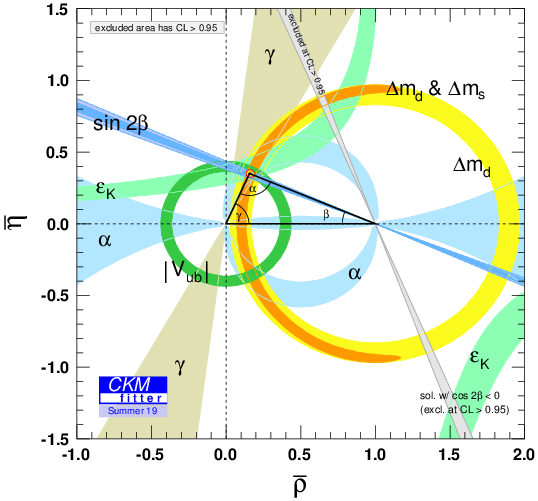
\includegraphics[height = 3cm, width = 4cm]{ckmfitter.png}}

\begin{document}

\begin{frame}
  \titlepage
\end{frame}

% These three lines create an automatically generated table of contents.
\begin{frame}{Outline}
  \tableofcontents
\end{frame}

\section{Introduction}
\begin{frame}{Introduction}
  \begin{figure}[H]
    \centering
    \vspace{0.3cm}
    \begin{subfigure}{0.5\textwidth}
      \centering
      \begin{fmffile}{fgraph/fgraph_BtoDK1}
        \setlength{\unitlength}{0.4cm}
        \begin{fmfgraph*}(6,6)
          \fmfstraight
          \fmfleft{i1,B,i2,t1,t2,t3,t9,t10}
          \fmfright{o1,D,o2,t4,t5,o3,K,o4}
          \fmflabel{$\bar{u}$}{i1}
          \fmflabel{$b$}{i2}
          \fmfv{l.d=20,l.a=180,l={$B^-$\mylbrace{30}{-8}}}{B}
          \fmflabel{$\bar{u}$}{o1}
          \fmflabel{$c$}{o2}
          \fmflabel{$\bar{u}$}{o3}
          \fmflabel{$s$}{o4}
          \fmfv{l.d=15,l.a=0,l={\myrbrace{30}{-12}}$D^0$}{D}
          \fmfv{l.d=15,l.a=0,l={\myrbrace{30}{11}}$K^-$}{K}
          \fmf{fermion}{o1,i1}
          \fmf{fermion,tension=1.5}{i2,v1}
          \fmf{fermion}{v1,o2}
          \fmf{phantom,tension=1.5}{t9,v2}
          \fmf{boson,label=$W$,label.side=left,tension=0}{v1,v2}
          \fmf{fermion}{v2,o4}
          \fmf{fermion}{o3,v2}
        \end{fmfgraph*}
      \end{fmffile}
      \vspace{0.5cm}
      \caption{$B^-\to D^0K^-$}
    \end{subfigure}%
    \begin{subfigure}{0.5\textwidth}
      \centering
      \begin{fmffile}{fgraph/fgraph_BtoDK2}
        \setlength{\unitlength}{0.4cm}
        \begin{fmfgraph*}(6,6)
          \fmfstraight
          \fmfleft{i1,t1,t2,B,t9,t10,i2}
          \fmfright{o1,K,o2,t4,t5,o3,D,o4}
          \fmflabel{$\bar{u}$}{i1}
          \fmflabel{$b$}{i2}
          \fmfv{l.d=20,l.a=180,l={$B^-$\mylbrace{100}{-8}}}{B}
          \fmflabel{$\bar{u}$}{o1}
          \fmflabel{$s$}{o2}
          \fmflabel{$\bar{c}$}{o3}
          \fmflabel{$u$}{o4}
          \fmfv{l.d=15,l.a=0,l={\myrbrace{30}{13}}$\bar{D^0}$}{D}
          \fmfv{l.d=15,l.a=0,l={\myrbrace{30}{-13}}$K^-$}{K}
          \fmf{fermion}{o1,i1}
          \fmf{fermion,tension=1.5}{i2,v1}
          \fmf{fermion}{v1,o4}
          \fmf{phantom,tension=1.5}{t2,v2}
          \fmf{boson,label=$W$,label.side=left,tension=0}{v1,v2}
          \fmf{fermion}{v2,o2}
          \fmf{fermion}{o3,v2}
        \end{fmfgraph*}
      \end{fmffile}
      \vspace{0.5cm}
      \caption{$B^-\to\bar{D^0}K^-$}
    \end{subfigure}
  \end{figure}
  \begin{center}
    $\gamma\equiv\text{arg}\Big(-\frac{V_{ud}V^*_{ub}}{V_{cd}V^*_{cb}}\Big)$ \\
    \vspace{0.3cm}
    $b\to u\bar{c}s$ and $b\to u\bar{u}s$ interference when $D^0$ and $\bar{D^0}$ decay into a common final state\\
    \vspace{0.3cm}
    In this analysis, consider $D\to K^+K^-\pi^+\pi^-$
  \end{center}
\end{frame}

\begin{frame}{Introduction}
  \begin{itemize}
    \item{CP observables:}
    \begin{itemize}
      \item{$x_\pm^{DK} = r_B^{DK}\cos(\delta_B^{DK}\pm\gamma)$}
      \item{$y_\pm^{DK} = r_B^{DK}\sin(\delta_B^{DK}\pm\gamma)$}
      \item{$x_\xi^{D\pi} = \Re(\xi^{D\pi})$, $y_\xi^{D\pi} = \Im(\xi^{D\pi})$ $\quad\quad\Big(\xi^{D\pi} = \frac{r_B^{D\pi}}{r_B^{DK}}e^{i(\delta_B^{D\pi} - \delta_B^{DK})}\Big)$}
    \end{itemize}
  \end{itemize}
  \begin{block}{Event yield in bin $i$}
    $N^-_i = h_{B^-}\Big(K_i + \big(x_-^2 + y_-^2\big)\bar{K_i} + 2\sqrt{K_i\bar{K_i}}\big(x_-c_i + y_-s_i\big)\Big)$
    $N^+_{-i} = h_{B^+}\Big(K_i + \big(x_+^2 + y_+^2\big)\bar{K_i} + 2\sqrt{K_i\bar{K_i}}\big(x_+c_i + y_+s_i\big)\Big)$
  \end{block}
  \begin{block}{Amplitude averaged strong phases and fractional yield}
    $c_i = \frac{\int_i\dd{\Phi}|\mathcal{A}(D^0)||\mathcal{A}(\bar{D^0})|\cos(\delta_D)}{\sqrt{\int_i\dd{\Phi}\abs{\mathcal{A}(D^0)}^2\int_i\dd{\Phi}\abs{\mathcal{A}(\bar{D^0})}^2}}, \quad K_i = \frac{\int_i\dd{\Phi}|\mathcal{A}(D^0)|^2}{\sum_j\int_j\dd{\Phi}\abs{\mathcal{A}(D^0)}^2}$
  \end{block}
\end{frame}

\section{Binning scheme}
\begin{frame}{Binning Scheme}
  \begin{center}
    {\huge Binning scheme}
  \end{center}
\end{frame}

\begin{frame}{Binning scheme}
  \begin{itemize}
    \setlength\itemsep{1.2em}
    \item{Use LHCb model (\href{https://arxiv.org/abs/1811.08304}{arXiv:1811.08304}) implemented in AmpGen}
    \item{Calculate $D^0$ and $\bar{D^0}$ amplitude from $D$ daughter momenta}
    \item{$\mathcal{A}(D^0)/\mathcal{A}(\bar{D^0}) = r_D\exp(i\delta_D)$}
    \item{Bin along $\delta_D$ to avoid dilution during averaging}
    \item{Enhance interference by separating bin $+i$ and $-i$ at $r_D = 1$}
    \item{Analogy from $K_S\pi^+\pi^-$: $m^2_+ = m^2_-$ separates CF and DCS resonances}
    \item{Maximize $Q = \frac{1}{2}(Q_+ + Q_-)$ by moving bin boundaries symmetrically around $\delta_D = 0$:}
  \end{itemize}
  \begin{equation*}
    Q_\pm^2 = 1 - \sum_i\frac{K_i\bar{K_i}(1 - c_i^2 - s_i^2)}{N^\pm_i}\Big/\sum_iK_i
  \end{equation*}
\end{frame}

\begin{frame}{Binning scheme}
  \begin{figure}
    \centering
    \vspace{-0.2cm}
    \begin{subfigure}{0.5\textwidth}
      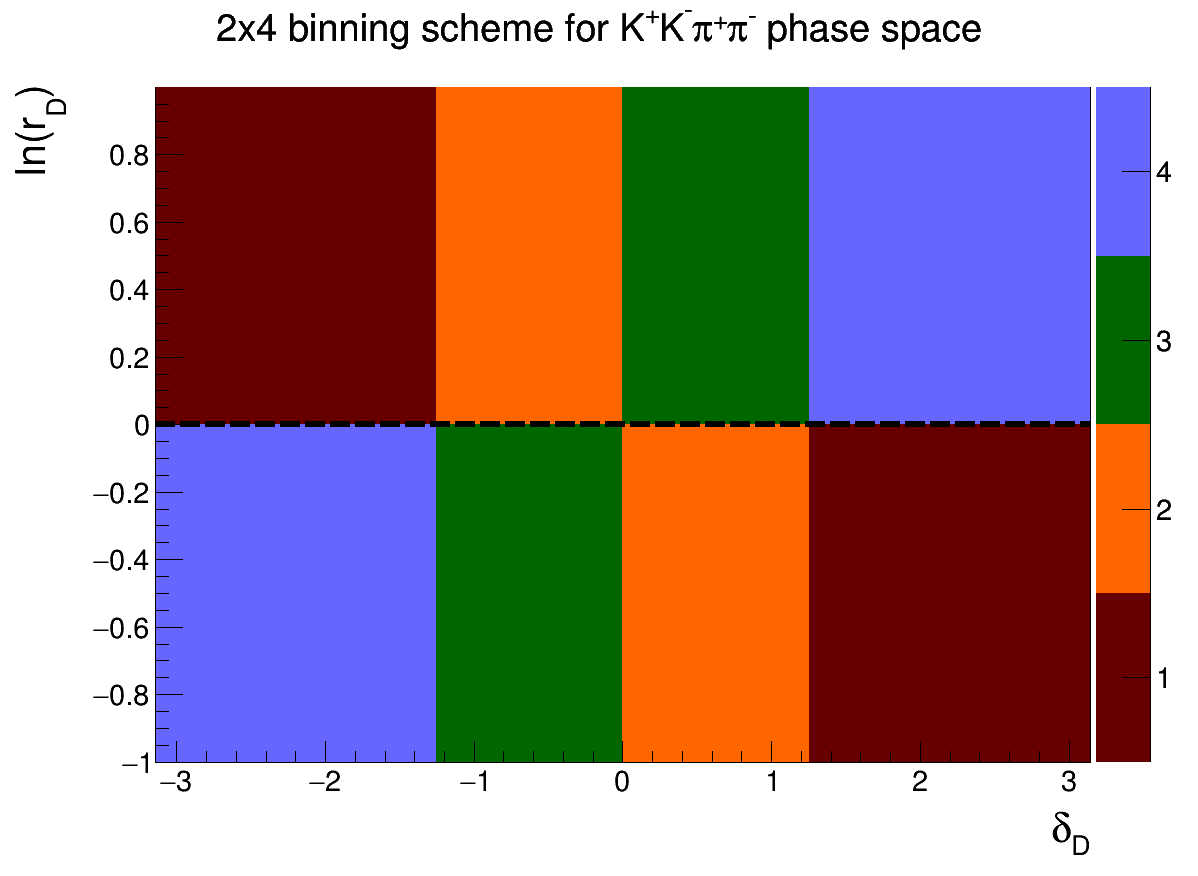
\includegraphics[width = 1.0\textwidth]{Plots/BinningScheme4BinsPlot.png}
      \caption{$2\times 4$ binning scheme \\ $Q = 0.85$}
    \end{subfigure}%
    \begin{subfigure}{0.5\textwidth}
      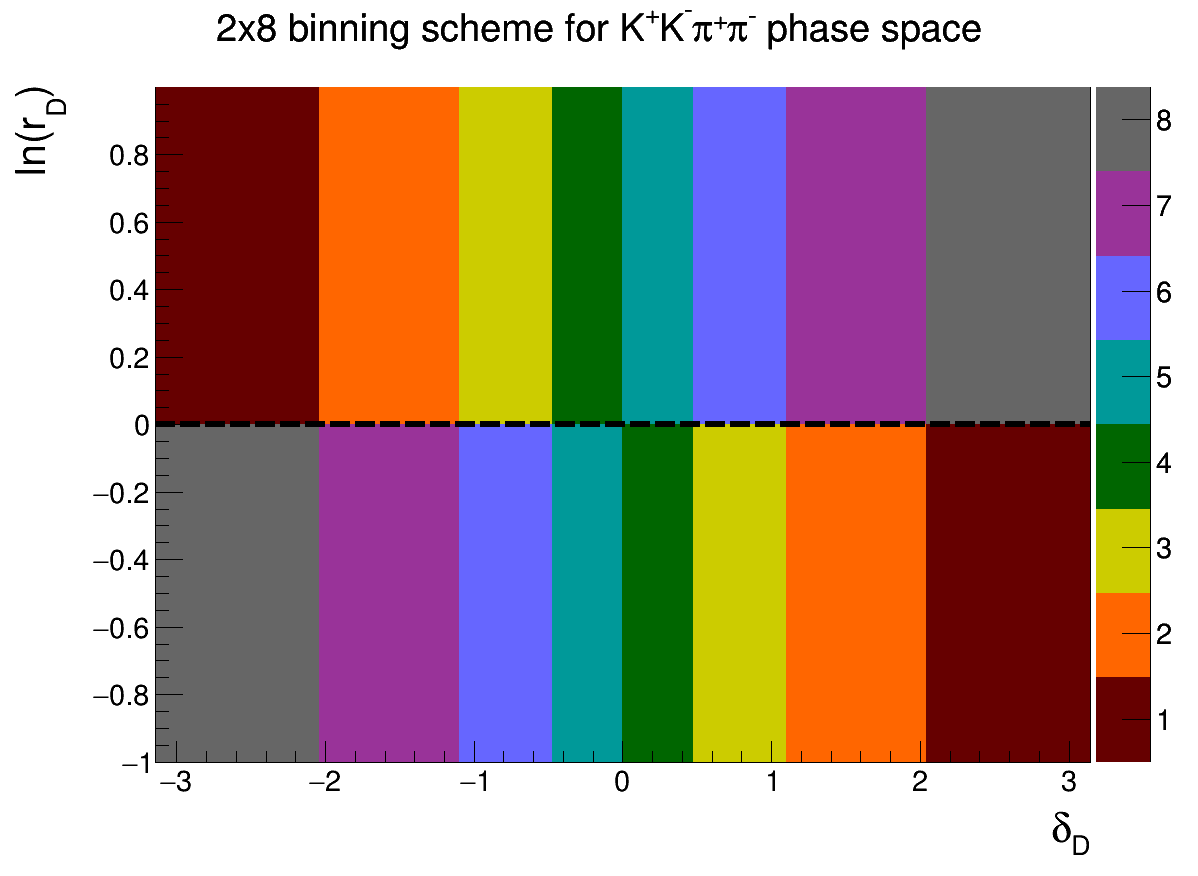
\includegraphics[width = 1.0\textwidth]{Plots/BinningScheme8BinsPlot.png}
      \caption{$2\times 8$ binning scheme \\ $Q = 0.90$}
    \end{subfigure}
  \end{figure}
\end{frame}

\begin{frame}{Strong phases}
  \begin{figure}
    \centering
    \vspace{-0.2cm}
    \begin{subfigure}{0.5\textwidth}
      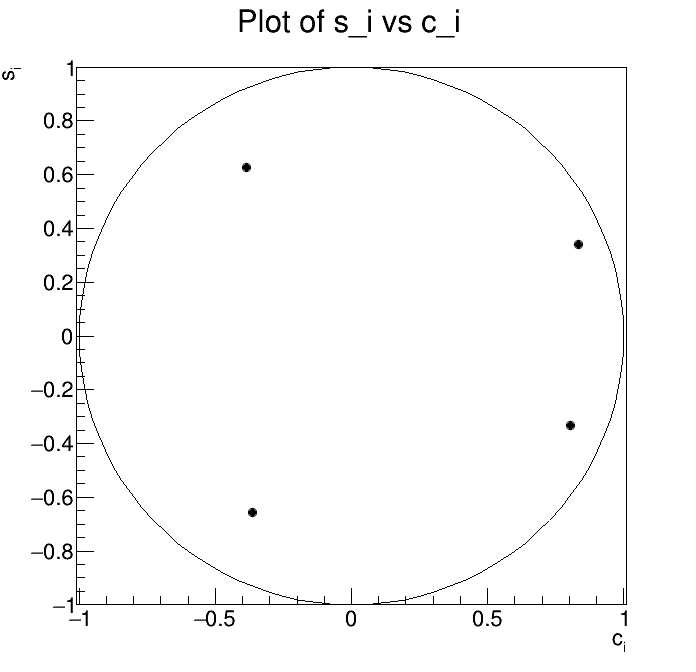
\includegraphics[width = 1.0\textwidth]{Plots/Amplitude_4bins_VariableBins_1p20923_50M_sample1_cs.png}
      \caption{$c_i$ and $s_i$ for the \\$2\times 4$ binning scheme}
    \end{subfigure}%
    \begin{subfigure}{0.5\textwidth}
      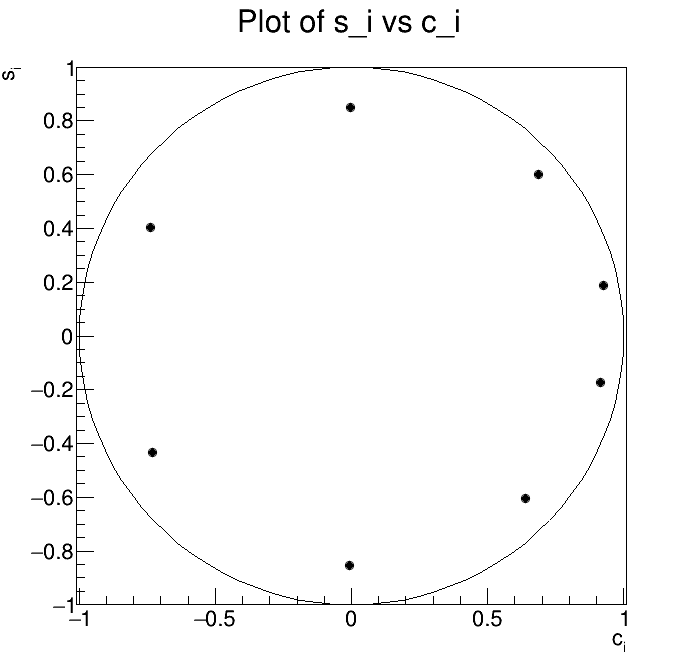
\includegraphics[width = 1.0\textwidth]{Plots/Amplitude_8bins_VariableBins_0p645101_1p72065_2p09644_50M_sample1_cs.png}
      \caption{$c_i$ and $s_i$ for the \\$2\times 8$ binning scheme}
    \end{subfigure}
  \end{figure}
\end{frame}

\begin{frame}{Fractional yields}
  \begin{figure}
    \centering
    \vspace{-0.2cm}
    \begin{subfigure}{0.5\textwidth}
      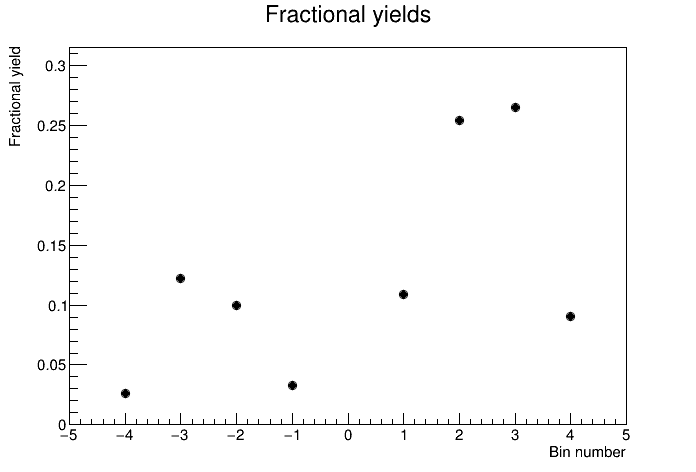
\includegraphics[width = 1.0\textwidth]{Plots/Amplitude_4bins_VariableBins_1p20923_50M_sample1_KKbar.png}
      \caption{$K_i$ for the \\$2\times 4$ binning scheme}
    \end{subfigure}%
    \begin{subfigure}{0.5\textwidth}
      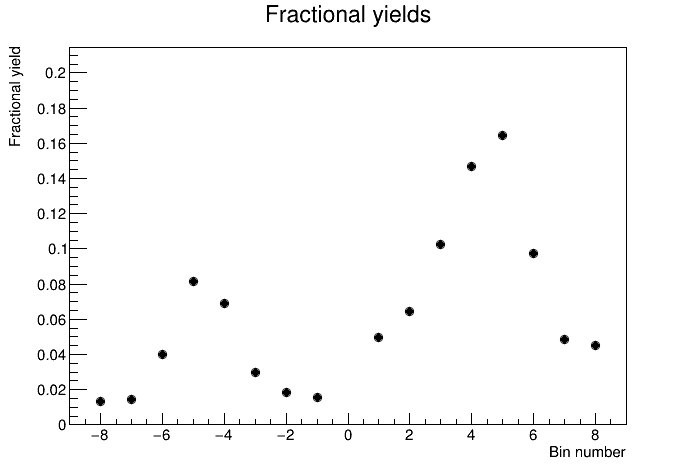
\includegraphics[width = 1.0\textwidth]{Plots/Amplitude_8bins_VariableBins_0p645101_1p72065_2p09644_50M_sample1_KKbar.png}
      \caption{$K_i$ for the \\$2\times 8$ binning scheme}
    \end{subfigure}
  \end{figure}
\end{frame}

\begin{frame}{Study of $\gamma$ precision}
  \begin{itemize}
    \item{Generate $2000$ $B^\pm$ candidates in AmpGen}
    \item{Unbinned fit benchmark: $\Delta\gamma = \SI{11}{\degree}$}
    \item{Both $2\times 4$ and $2\times 8$ binning schemes are consistent with their $Q$ values}
  \end{itemize}
  \begin{figure}
    \centering
    \vspace{-0.2cm}
    \begin{subfigure}{0.5\textwidth}
      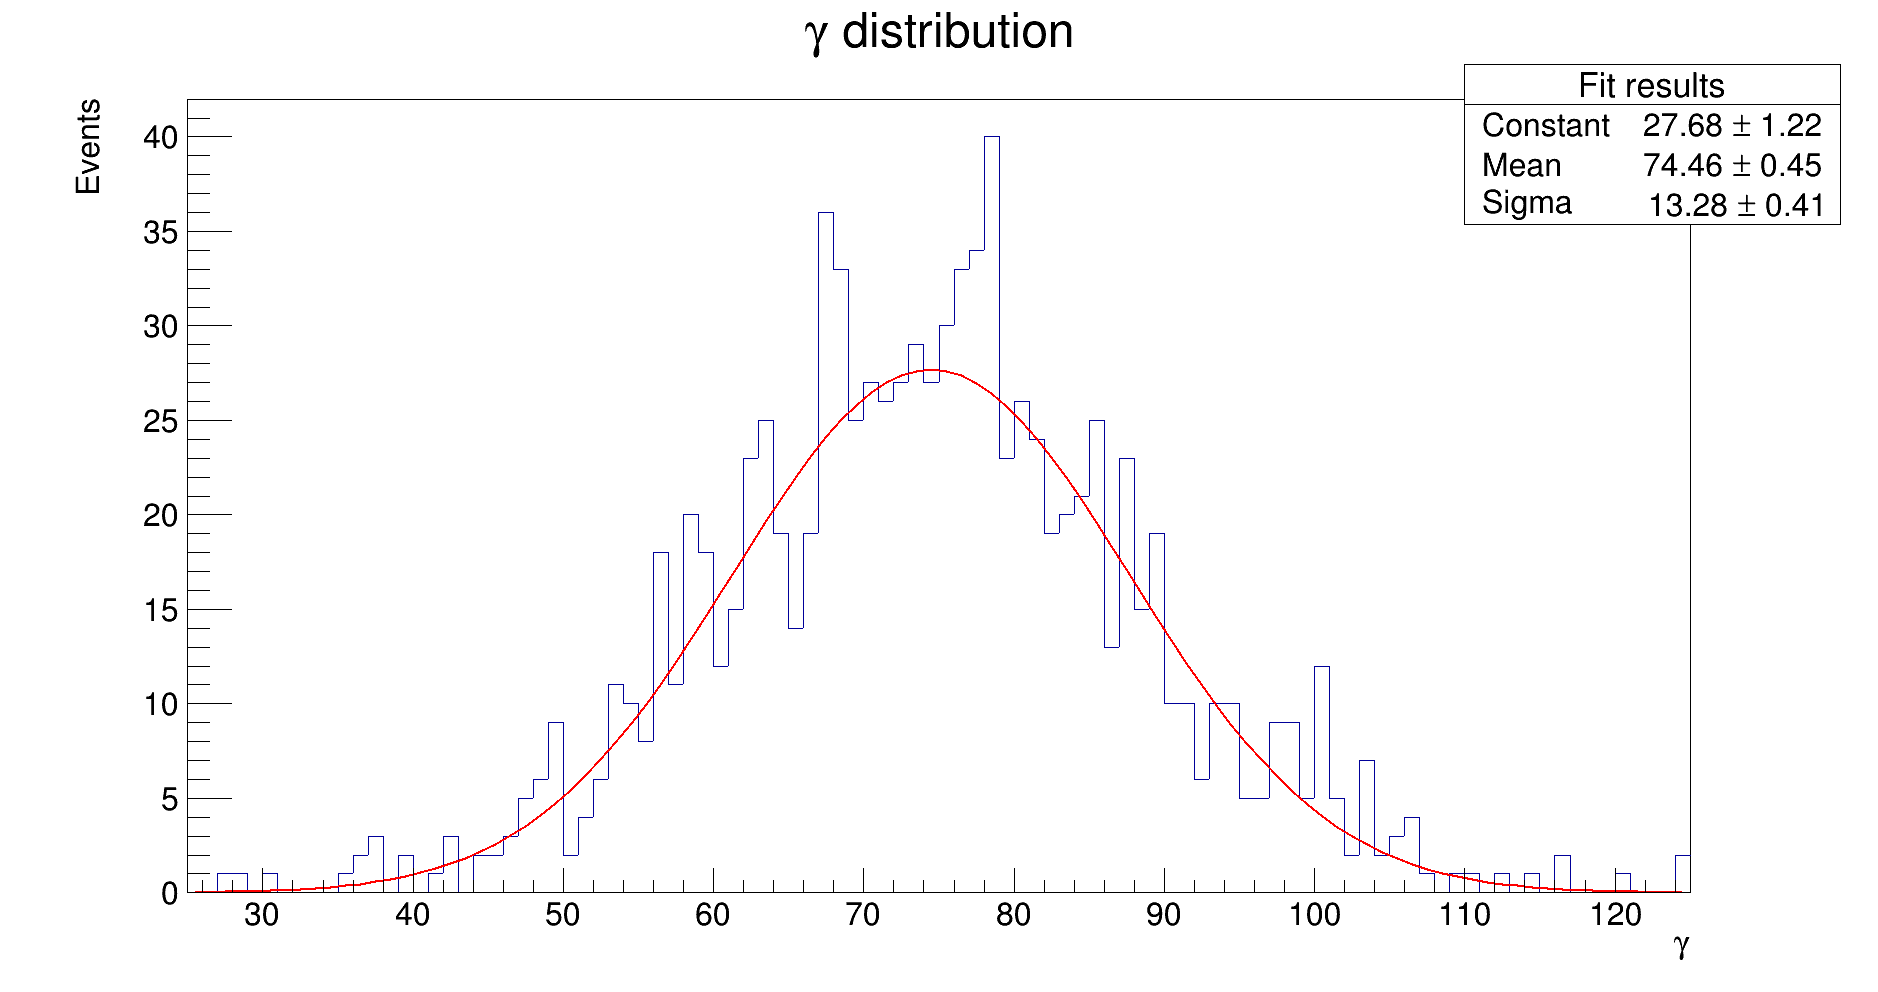
\includegraphics[width = 1.0\textwidth]{Plots/GammaDistribution4BinsVariableWidth.png}
      \caption{$2\times 4$ binning scheme \\ $\Delta\gamma = \SI{13}{\degree}$}
    \end{subfigure}%
    \begin{subfigure}{0.5\textwidth}
      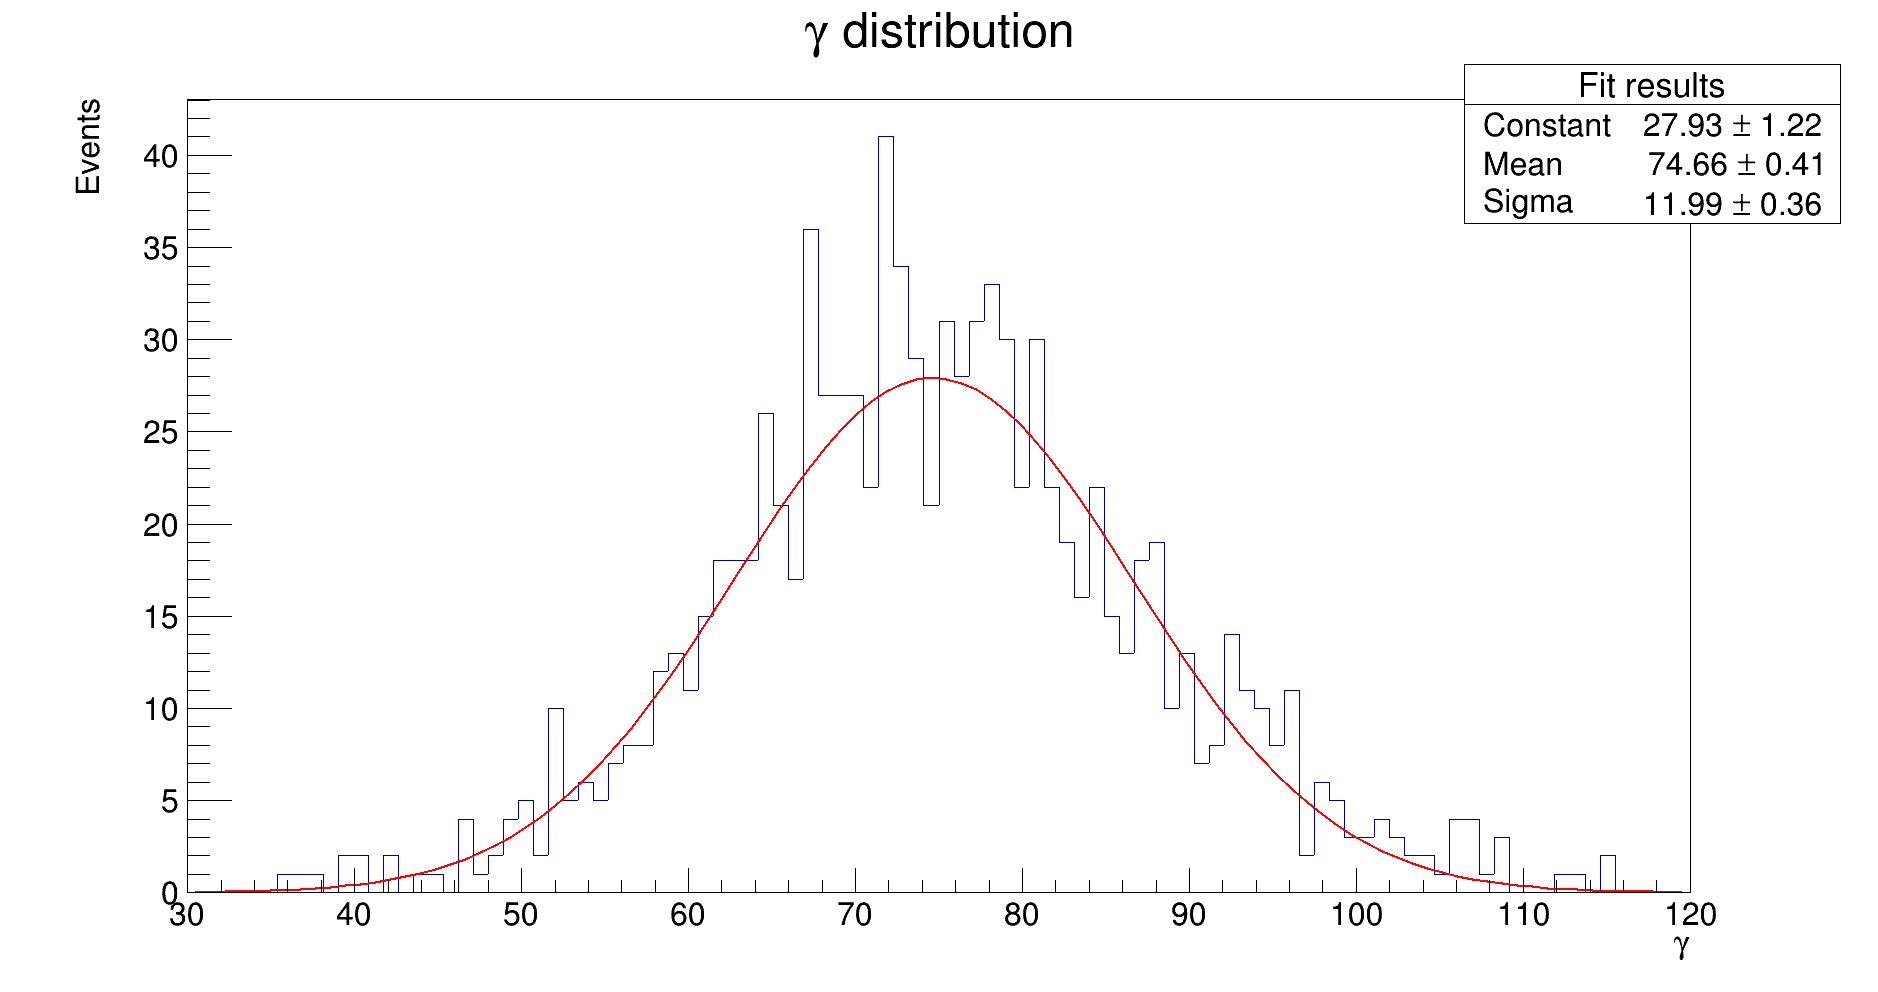
\includegraphics[width = 1.0\textwidth]{Plots/GammaDistribution8BinsVariableWidth.png}
      \caption{$2\times 8$ binning scheme \\ $\Delta\gamma = \SI{12}{\degree}$}
    \end{subfigure}
  \end{figure}
\end{frame}

\section{\texorpdfstring{$B^\pm\to(K^+K^-\pi^+\pi^-)_Dh^\pm$}{B to K+ K- pi+ pi- h} selection}
\begin{frame}{$B^\pm\to(K^+K^-\pi^+\pi^-)_Dh^\pm$ selection}
  \begin{center}
    {\huge $B^\pm\to(K^+K^-\pi^+\pi^-)_Dh^\pm$ selection}
  \end{center}
\end{frame}

\begin{frame}{Samples}
  \begin{itemize}
    \setlength\itemsep{1.2em}
    \item{Stripping lines:}
    \begin{itemize}
      \item{$\text{StrippingB2D0PiD2HHHHBeauty2CharmLineDecision}$}
      \item{$\text{StrippingB2D0KD2HHHHBeauty2CharmLineDecision}$}
    \end{itemize}
    \item{Data samples: 2015-2018 (2011-2012 not processed yet)}
    \item{MC samples: 2016-2018, filtered, AmpGen}
  \end{itemize}
\end{frame}

\begin{frame}{Initial cuts}
  \begin{center}
    Trigger requirements identical to that of LHCb-ANA-2020-001
  \end{center}
  \centering
  \def\arraystretch{1.2}%
  \begin{tabular}{|l|l|}
    \hline
    Run 1 trigger        & (\texttt{Bu\_L0Global\_TIS} or \texttt{Bu\_L0HadronDecision\_TOS}) \\
    requirements         & and (\texttt{Bu\_Hlt1TrackAllL0Decision\_TOS}) \\
                         & and (\texttt{Bu\_Hlt2Topo2BodyBBDTDecision\_TOS} or \\
                         & \texttt{Bu\_Hlt2Topo3BodyBBDTDecision\_TOS} or \\
                         & \texttt{Bu\_Hlt2Topo4BodyBBDTDecision\_TOS}) \\
    \hline
    Run 2 trigger        & (\texttt{Bu\_L0Global\_TIS} or \texttt{Bu\_L0HadronDecision\_TOS}) \\
    requirements         & and (\texttt{Bu\_Hlt1TrackMVADecision\_TOS} or \\
                         & \texttt{Bu\_Hlt1TwoTrackMVADecision\_TOS}) \\
                         & and (\texttt{Bu\_Hlt2Topo2BodyDecision\_TOS} or \\
                         & \texttt{Bu\_Hlt2Topo3BodyDecision\_TOS} or \\
                         & \texttt{Bu\_Hlt2Topo4BodyDecision\_TOS}) \\
    \hline
  \end{tabular}
\end{frame}

\begin{frame}{Initial cuts}
  \begin{center}
    Rectangular cuts before BDT
  \end{center}
  \centering
  \def\arraystretch{1.2}%
  \begin{tabular}{|l|l|}
    \hline
    Standard cuts                     & Value \\
    \hline
    Bachelor momentum $p$             & $< \SI{100}{\giga\eV}$ \\
    Bachelor has RICH                 & True \\
    $K^\pm$ from $D$ momentum $p$     & $< \SI{100}{\giga\eV}$ \\
    $K^\pm$ has RICH                  & True \\
    $D$ invariant mass                & Within $\pm\SI{25}{\mega\eV}$ of $m_{D^0}^\text{PDG}$ \\
    DecayTreeFitter (DTF) convergence & True \\
    $B^\pm$ DTF mass range            & $[5080, 5800]\si{\mega\eV}$ \\
    \hline
  \end{tabular}
\end{frame}

\begin{frame}{Boosted Decision Tree}
  \begin{itemize}
    \setlength\itemsep{1.2em}
    \item{BDTG from TMVA Toolkit}
    \item{Signal sample: $B^\pm\to DK^\pm$ and $B^\pm\to D\pi^\pm$ MC samples}
    \item{Background sample: $B^\pm\to D\pi^\pm$ using $m_{B^\pm}^\text{DTF}\in[5800, 7000]\si{\mega\eV}$}
  \end{itemize}
\end{frame}

\begin{frame}{BDT training particles}
  \begin{center}
    BDT training variables part 1
  \end{center}
  \centering
  %\def\arraystretch{1.2}%
  \begin{tabular}{|l|l|l|}
    \hline
    Name & Rank ($\%$) & Description \\
    \hline
    \texttt{log(D0\_RHO\_BPV)} & $7.7$ & $D$ radial distance to beamline \\
    \texttt{log(Bu\_FDCHI2\_OWNPV)} & $6.3$ & $B^\pm$ flight distance $\chi^2$ \\
    \texttt{log(Bu\_RHO\_BPV)} & $6.1$ & $B^\pm$ radial distance to beamline \\
    \texttt{log(Bach\_PT)} & $6.1$ & Bachelor transverse momentum \\
    \texttt{Bu\_PTASY\_1.5} & $5.3$ & $B^\pm$ asymmetry parameter \\
    \texttt{log(1-D0\_DIRA\_BPV)} & $5.0$ & Angle between PV and $D$ \\
    \texttt{log(Bu\_IPCHI2\_OWNPV)} & $4.8$ & $B^\pm$ impact parameter $\chi^2$ \\
    \texttt{log(1-Bu\_DIRA\_BPV)} & $4.7$ & Angle between PV and $B^\pm$ \\
    \texttt{log(h[1,2]\_PT)} & $4.4$ & $K^\pm$ transverse momentum \\
    \texttt{Bu\_MAXDOCA} & $4.4$ & $B^\pm$ distance of closest approach \\
    \texttt{log(Bach\_IPCHI2\_OWNPV)} & $4.1$ & Bachelor impact parameter $\chi^2$ \\
    \hline
  \end{tabular}
\end{frame}

\begin{frame}{BDT training particles}
  \begin{center}
    BDT training variables part 2
  \end{center}
  \centering
  %\def\arraystretch{1.2}%
  \begin{tabular}{|l|l|l|}
    \hline
    Name & Rank ($\%$) & Description \\
    \hline
    \texttt{log(Bu\_constD0PV\_D0\_P)} & $3.7$ & $D$ momentum from DTF \\
    \texttt{log(D0\_VTXCHI2DOF)} & $3.3$ & $D0$ vertex fit $\chi^2$ \\
    \texttt{log(h[3,4]\_IPCHI2\_OWNPV)} & $3.3$ & $\pi^\pm$ impact parameter $\chi^2$ \\
    \texttt{log(D0\_IPCHI2\_OWNPV)} & $3.2$ & $D$ impact parameter $\chi^2$ \\
    \texttt{log(h[3,4]\_PT)} & $3.2$ & $\pi^\pm$ transverse momentum \\
    \texttt{log(Bu\_PT)} & $2.8$ & $B^\pm$ transverse momentum \\
    \texttt{log(h[1,2]\_P)} & $2.8$ & $K^\pm$ momentum \\
    \texttt{log(Bach\_P)} & $2.7$ & Bachelor momentum \\
    \texttt{log(Bu\_constD0PV\_P)} & $2.6$ & $B^\pm$ momentum from DTF \\
    \texttt{log(h[1,2]\_IPCHI2\_OWNPV)} & $2.5$ & $K^\pm$ impact parameter $\chi^2$ \\
    \texttt{D0\_MAXDOCA} & $2.5$ & $D$ distance of closest approach \\
    \texttt{log(Bu\_VTXCHI2DOF)} & $2.0$ & $B^\pm$ vertex fit $\chi^2$ \\
    \texttt{log(h[3,4]\_P)} & $1.9$ & $\pi^\pm$ momentum \\
    \hline
  \end{tabular}
\end{frame}

\begin{frame}{BDT training results}
  \begin{figure}
    \centering
    \vspace{-0.2cm}
    \begin{subfigure}{0.5\textwidth}
      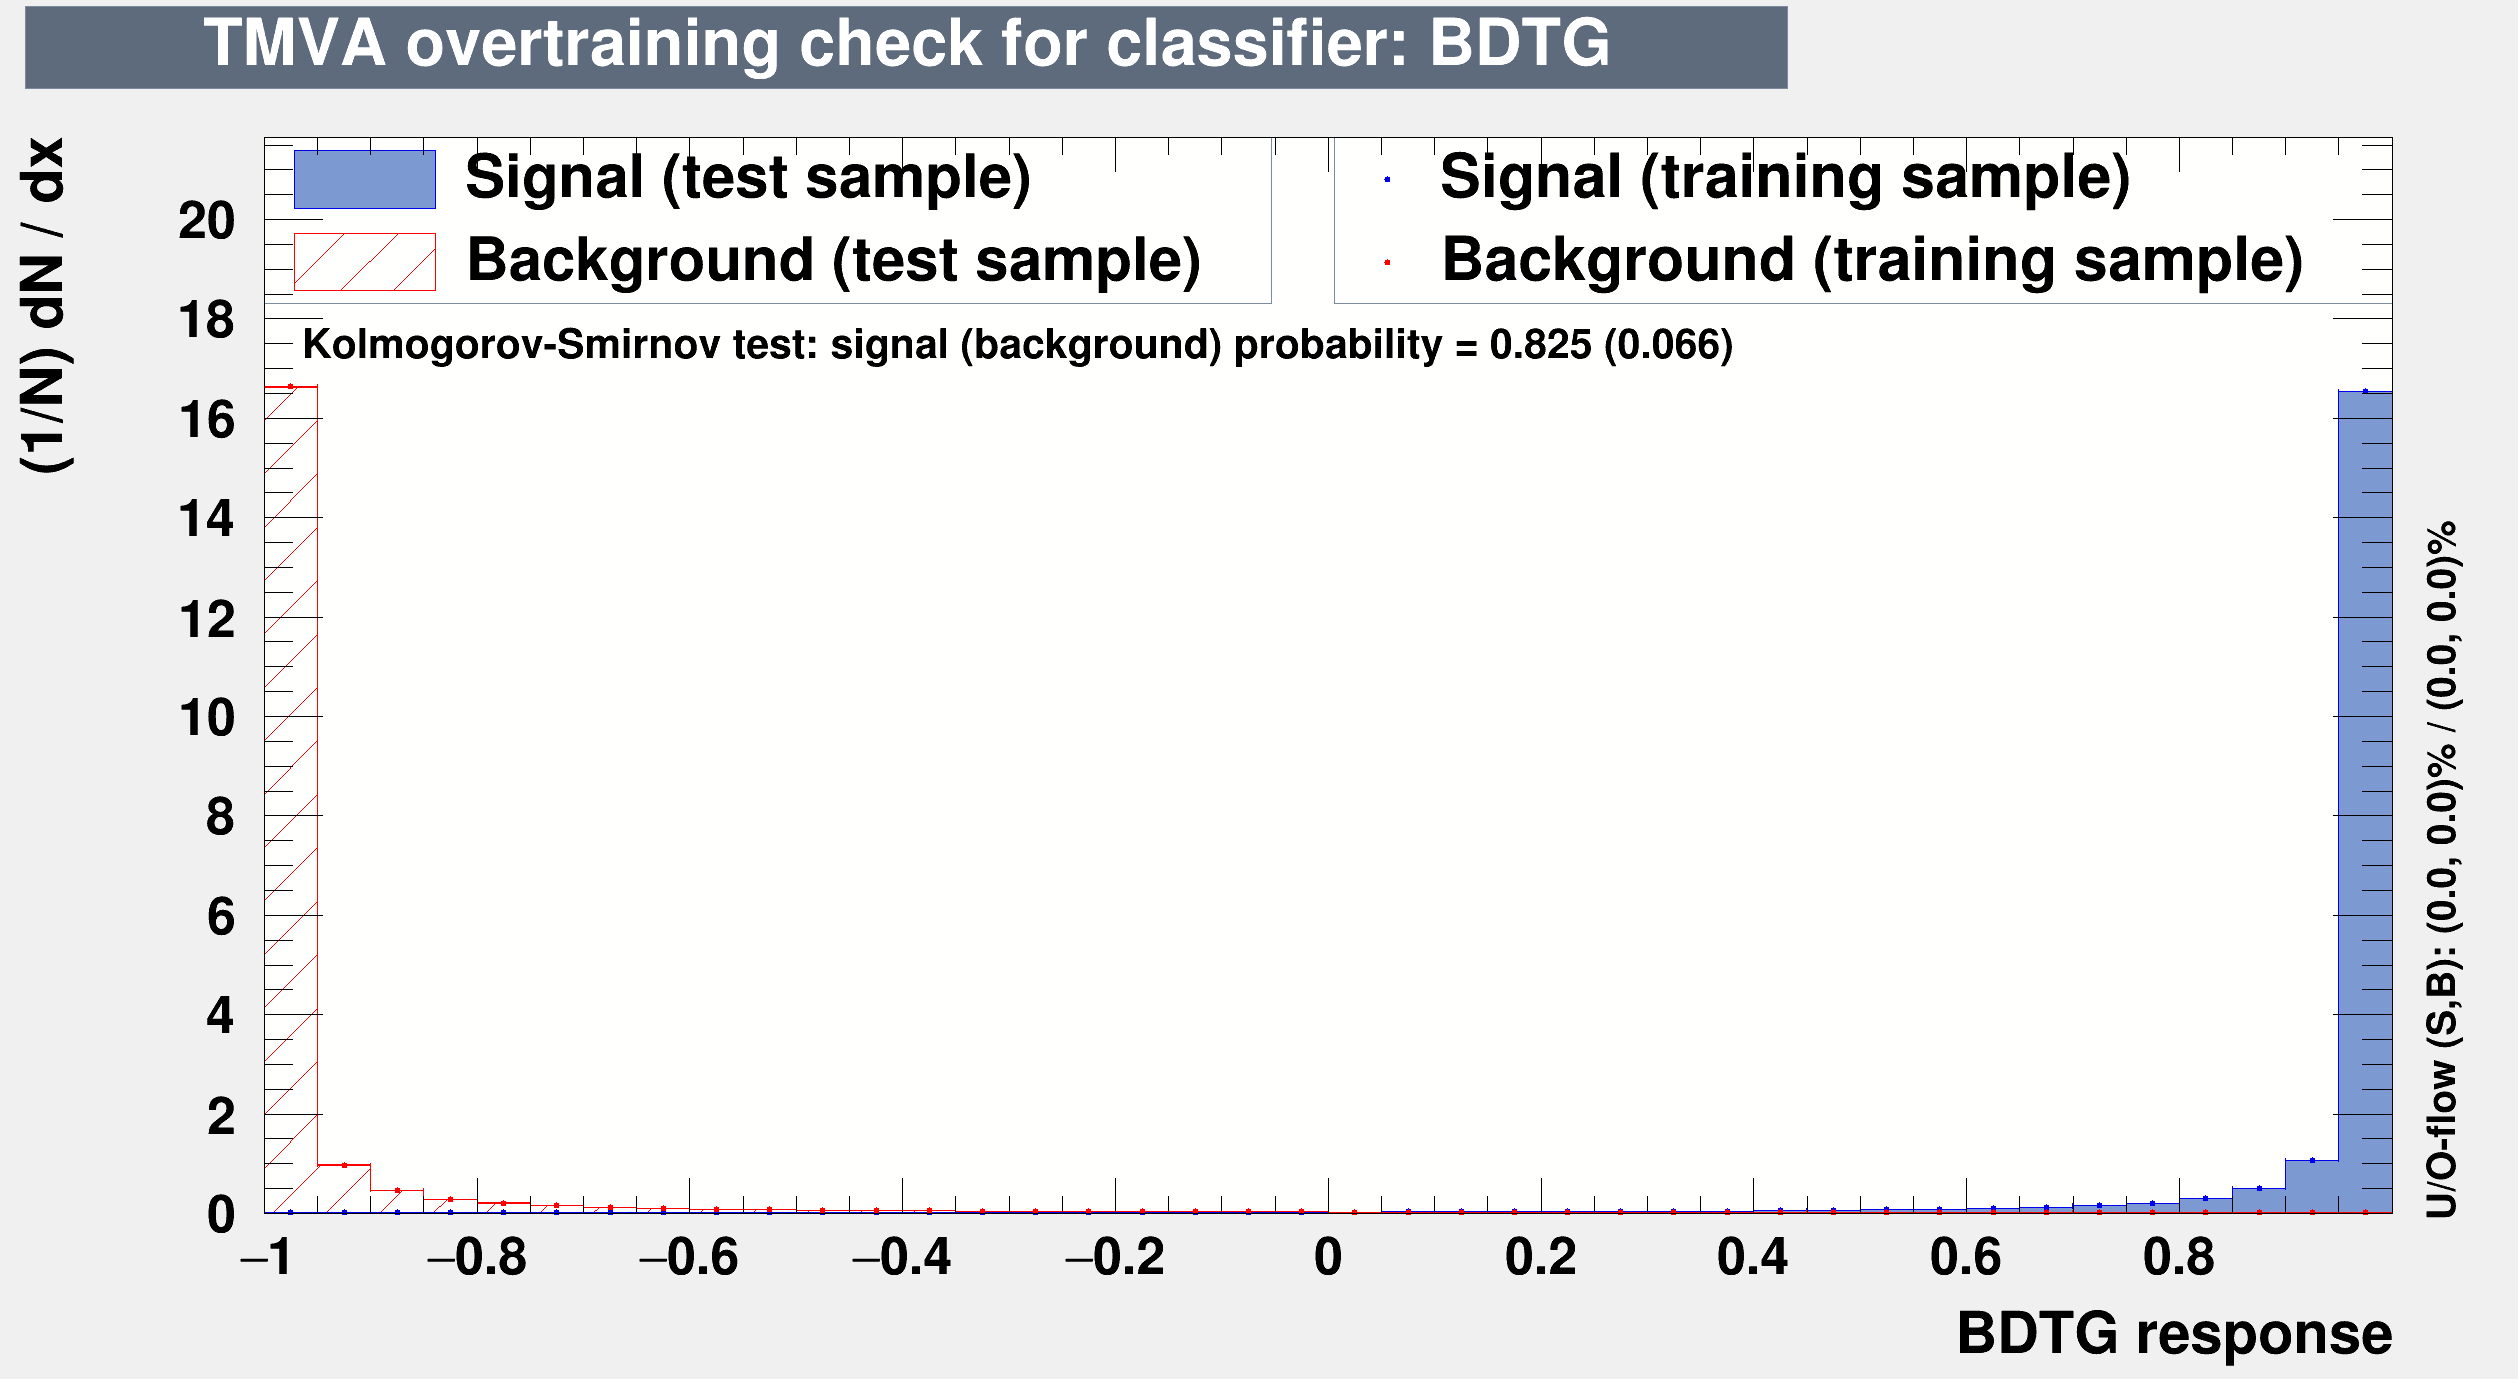
\includegraphics[width = 1.0\textwidth]{Plots/BDToutput.png}
      \caption{BDT output}
    \end{subfigure}%
    \begin{subfigure}{0.5\textwidth}
      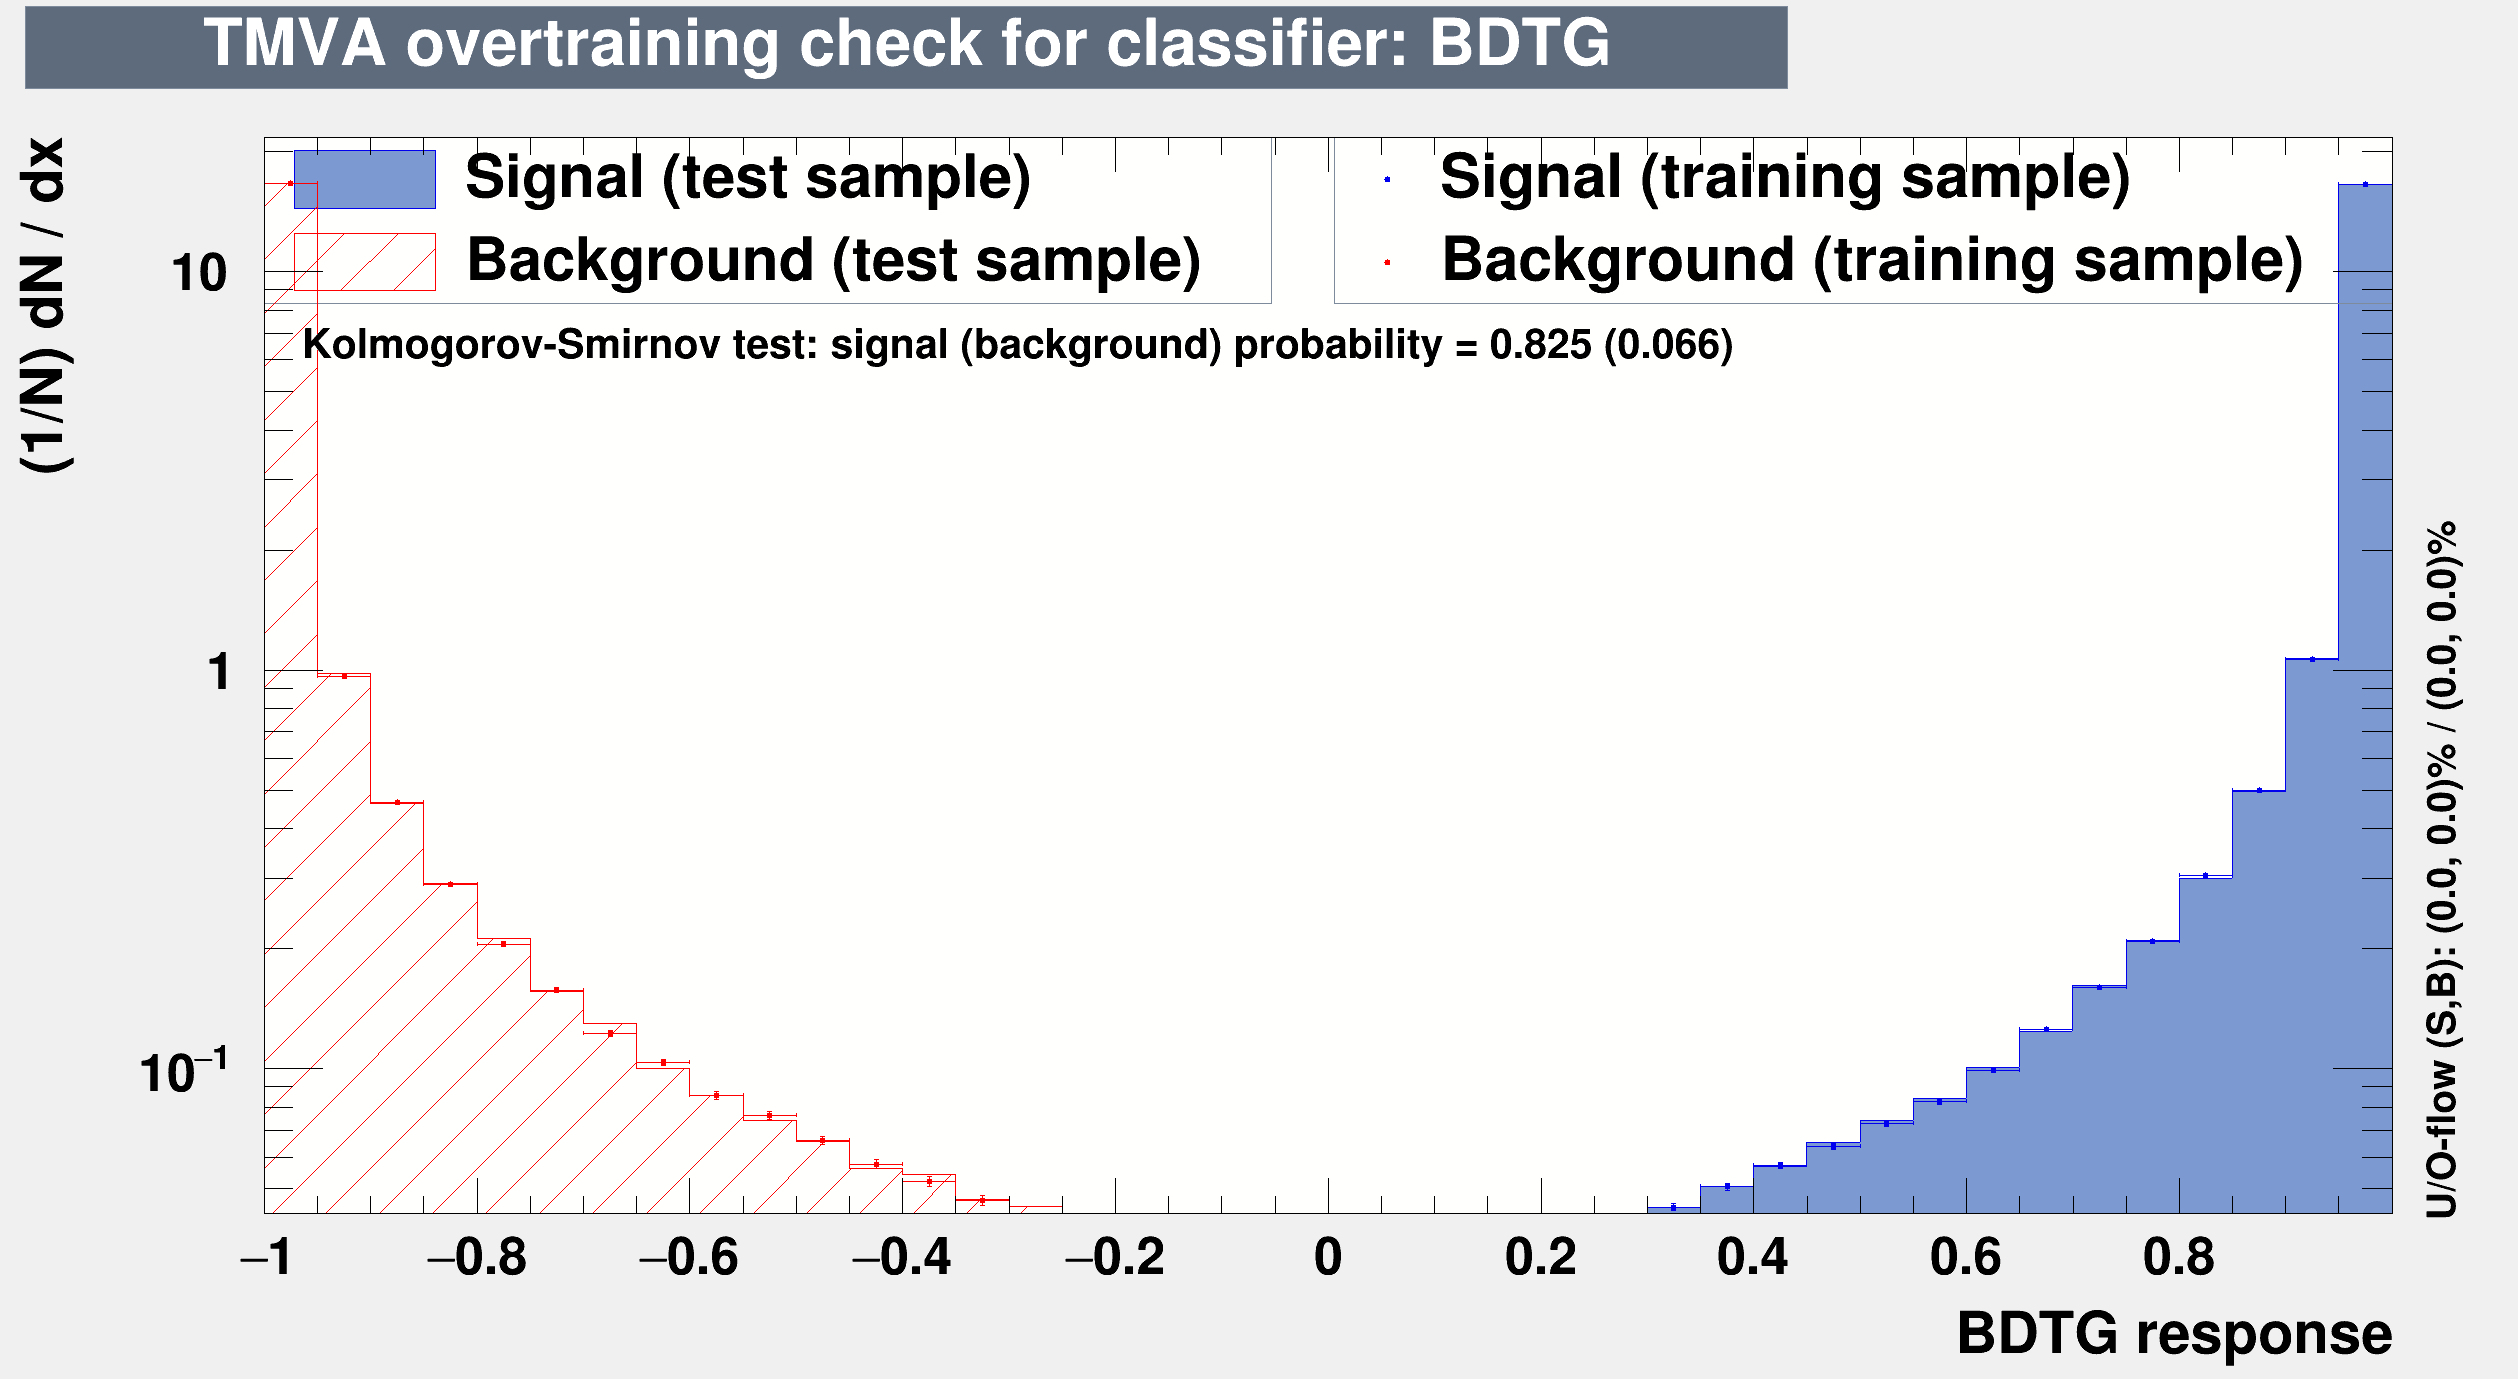
\includegraphics[width = 1.0\textwidth]{Plots/BDToutputLog.png}
      \caption{BDT output on a logarithmic scale}
    \end{subfigure}
  \end{figure}
\end{frame}

\begin{frame}{Charmless backgrounds from \texorpdfstring{$B^\pm\to K^+K^-\pi^+\pi^-K^\pm$}{B to K K pi pi K}}
  \begin{itemize}
    \item{Remove cut on DTF $\chi^2$}
    \item{Look in the $D$ mass sideband $[1770, 1820]\si{\mega\eV}$}
  \end{itemize}
  \begin{figure}
    \centering
    \vspace{-0.2cm}
    \begin{subfigure}{0.5\textwidth}
      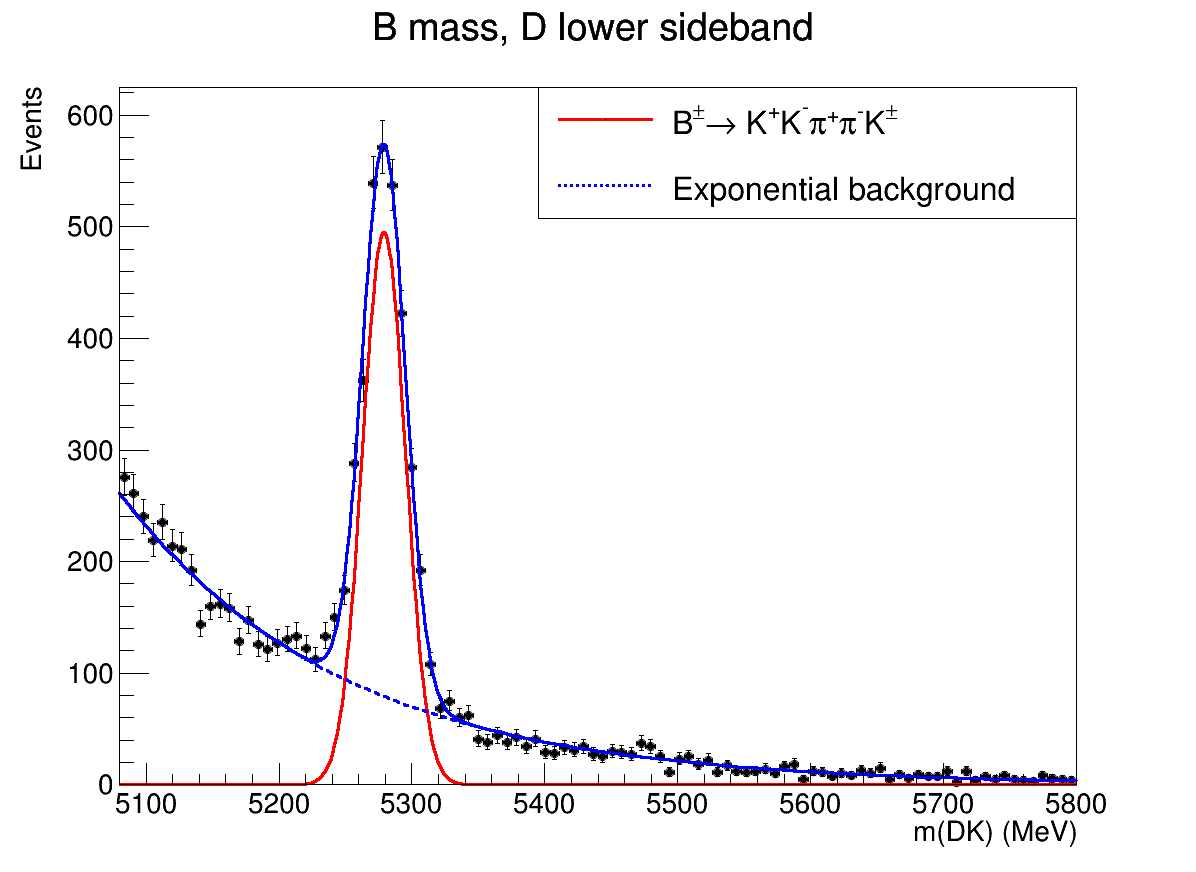
\includegraphics[width = 1.0\textwidth]{Plots/B2DKLower_Charmless.png}
      \caption{No flight significance cut \\ Yield: $\SI{2605(57)}{}$}
    \end{subfigure}%
    \begin{subfigure}{0.5\textwidth}
      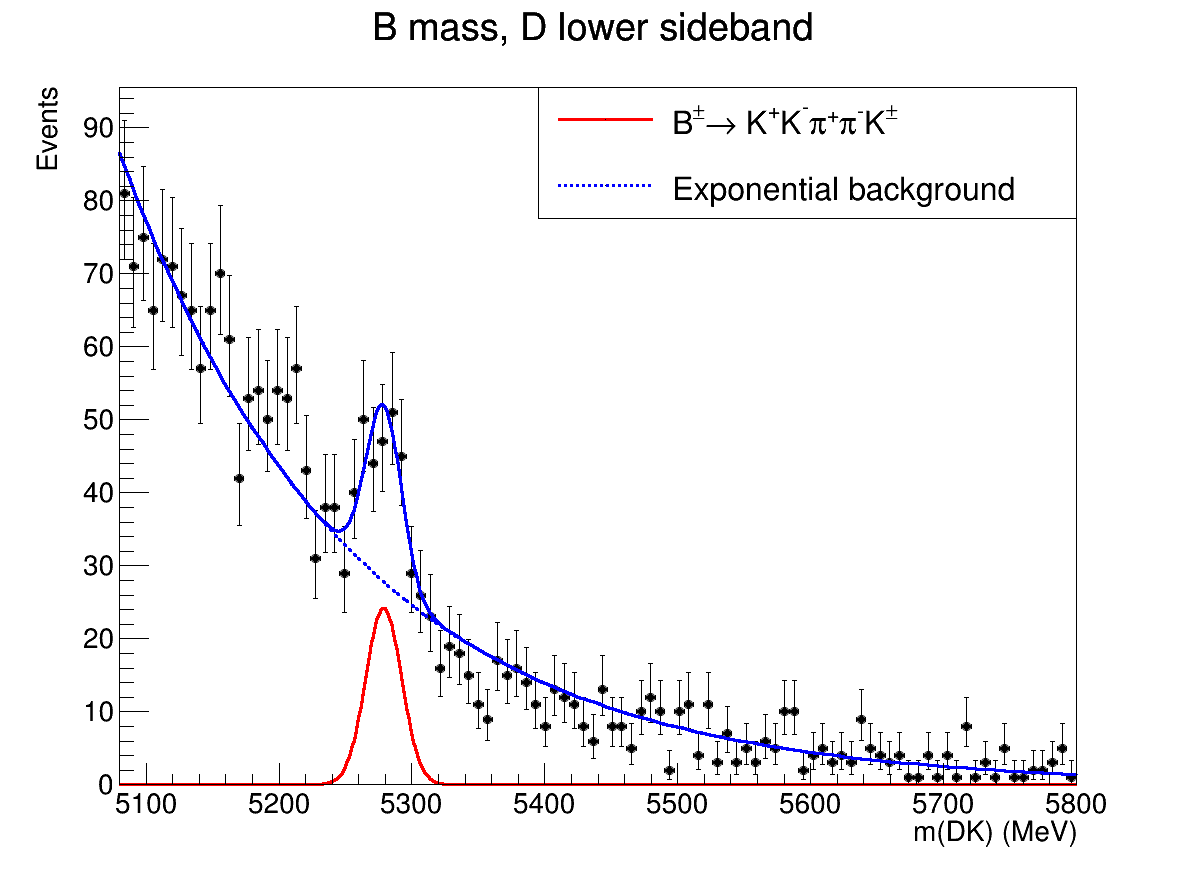
\includegraphics[width = 1.0\textwidth]{Plots/B2DKLowerFDCut_Charmless.png}
      \caption{Flight significance cut at $2$ \\ Yield: $\SI{110(19)}{}$}
    \end{subfigure}
  \end{figure}
  \begin{itemize}
    \item{Choose flight significance cut at $2$}
    \item{A cut larger than $\approx 3$ gives a charmless yield consistent with $0$}
  \end{itemize}
\end{frame}

\begin{frame}{Charmless backgrounds from \texorpdfstring{$B^\pm\to K^+K^-\pi^+\pi^-\pi^\pm$}{B to K K pi pi pi}}
  \begin{figure}
    \centering
    \vspace{-0.2cm}
    \begin{subfigure}{0.5\textwidth}
      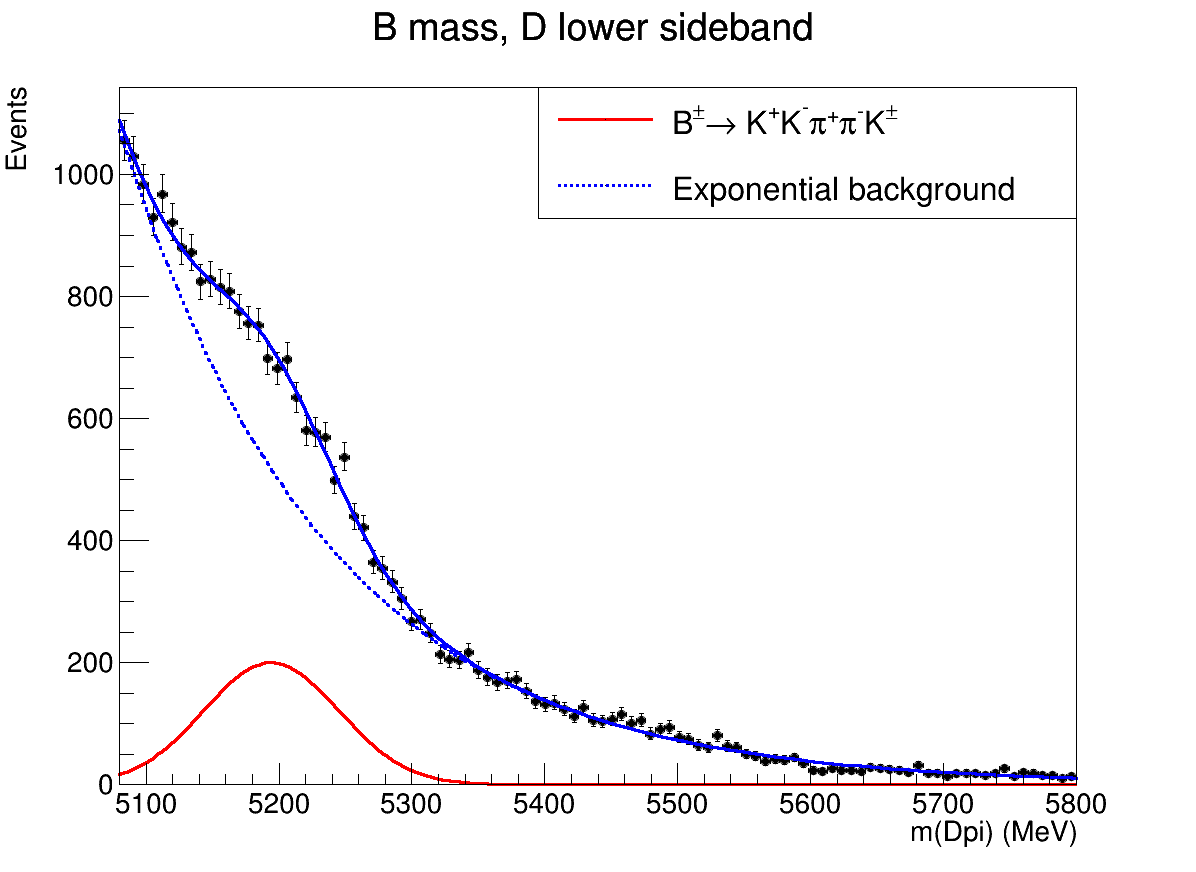
\includegraphics[width = 1.0\textwidth]{Plots/B2DpiLower_Charmless.png}
      \caption{No flight significance cut}
    \end{subfigure}%
    \begin{subfigure}{0.5\textwidth}
      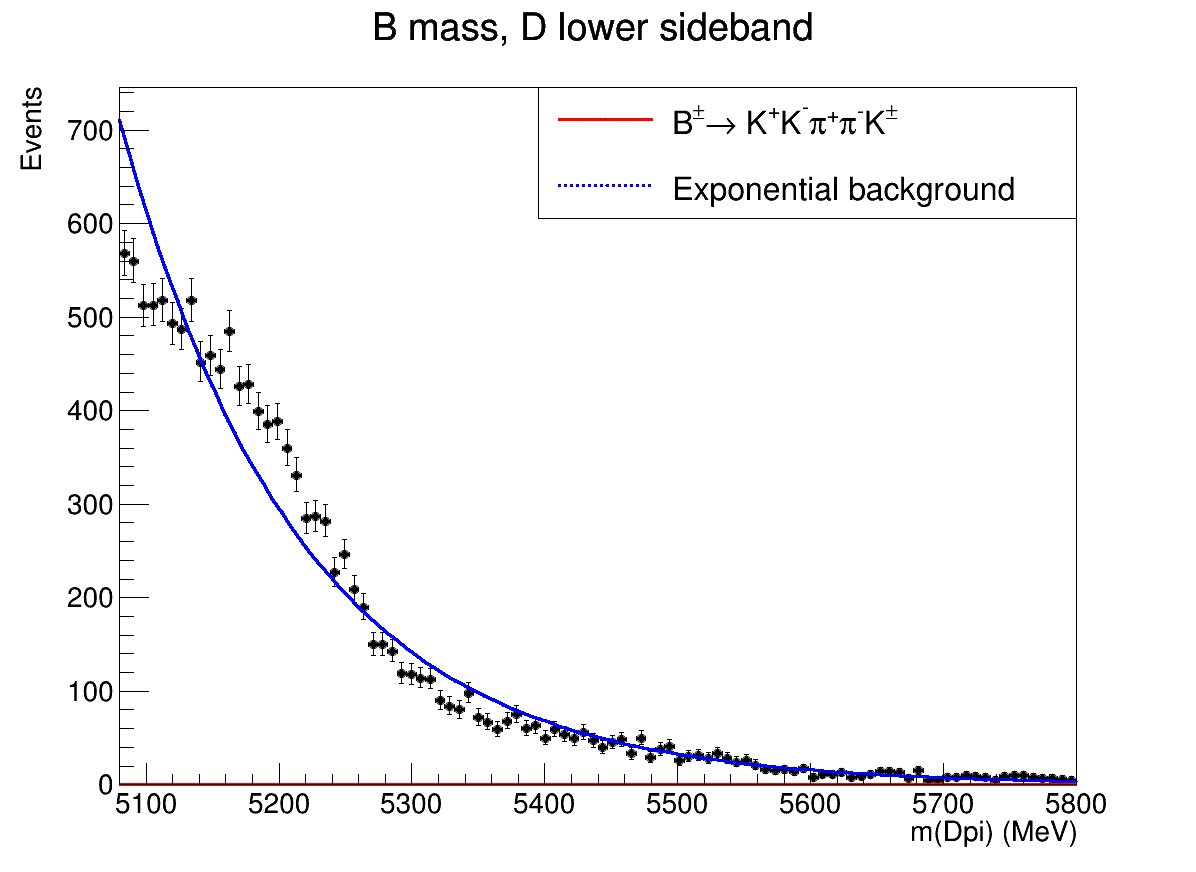
\includegraphics[width = 1.0\textwidth]{Plots/B2DpiLowerFDCut_Charmless.png}
      \caption{Flight significance cut at $2$}
    \end{subfigure}
  \end{figure}
  \begin{itemize}
    \item{No charmless background observed in the $B^\pm\to D\pi^\pm$ channel!}
  \end{itemize}
\end{frame}

\begin{frame}{Mis-ID background from \texorpdfstring{$B^\pm\to(K\pi\pi\pi)_Dh^\pm$}{B to K pi pi pi h}}
  \begin{itemize}
    \item{Study using MC samples from 2018}
    \item{Yields have been scaled to account for differences in sample size and branching fractions}
    \item{$\pi\pi\pi\pi$ background is negligible}
  \end{itemize}
  \begin{figure}
    \centering
    \vspace{-0.2cm}
    \begin{subfigure}{0.5\textwidth}
      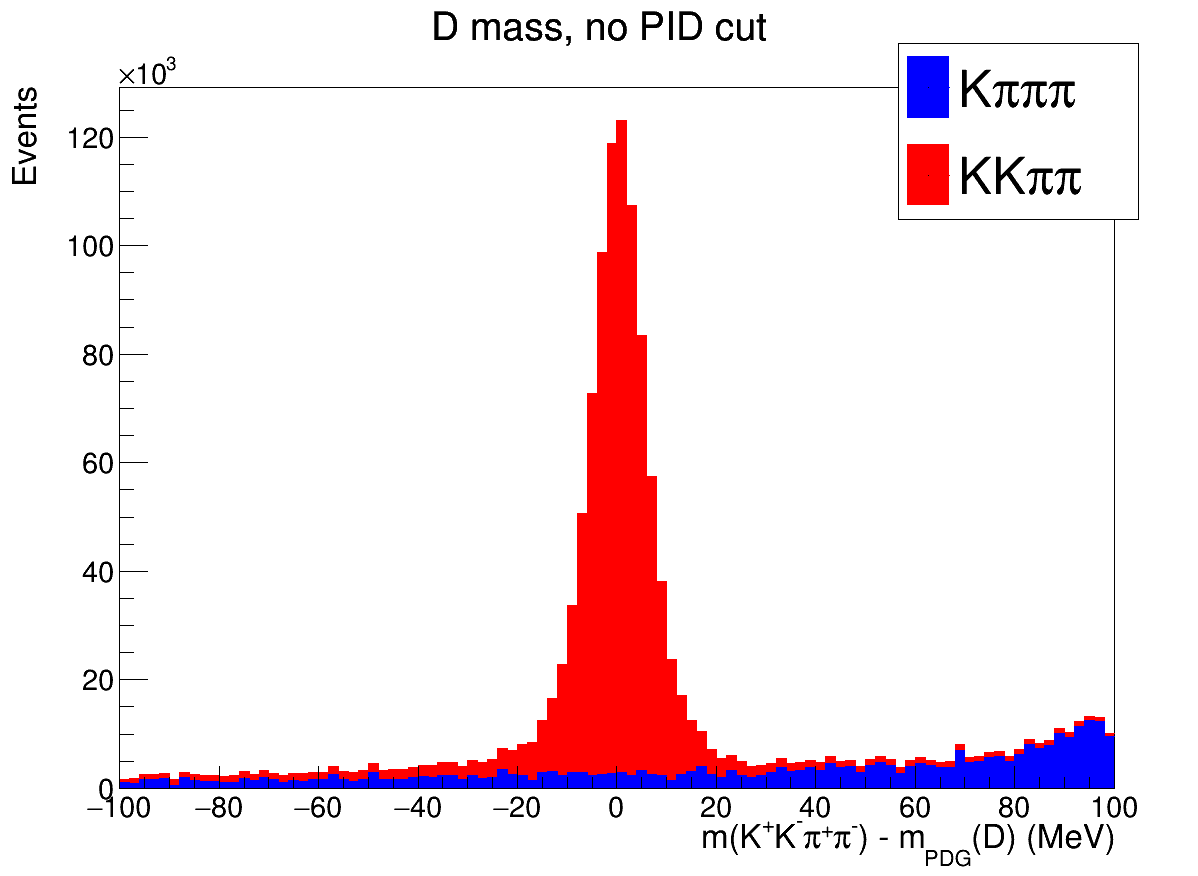
\includegraphics[width = 1.0\textwidth]{Plots/B2DK_Dmass_Background.png}
      \caption{$D$ invariant mass distribution}
    \end{subfigure}%
    \begin{subfigure}{0.5\textwidth}
      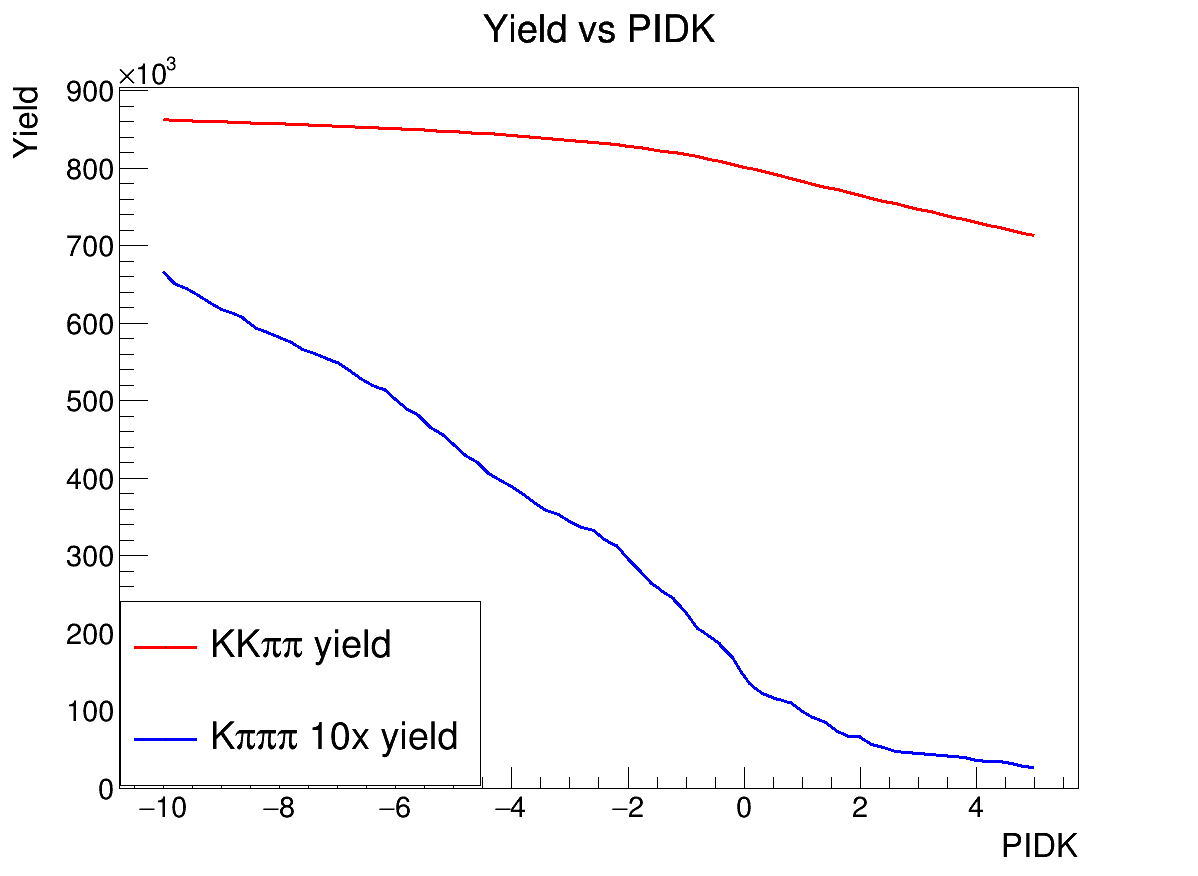
\includegraphics[width = 1.0\textwidth]{Plots/YieldVSPIDK.png}
      \caption{Signal and $K\pi\pi\pi$ background yield}
    \end{subfigure}
  \end{figure}
  \begin{itemize}
    \item{A cut at $\text{PIDK} > 0$ reduces the contamination from $7.2\%$ to $1.8\%$}
  \end{itemize}
\end{frame}

\begin{frame}{Final cuts}
  \begin{center}
    Cuts after BDT training
  \end{center}
  \centering
  \def\arraystretch{1.2}%
  \begin{tabular}{|l|l|}
    \hline
    Background suppression cuts & Value \\
    \hline
    BDTG                        & $< 0.75$ \\
    Bachelor PID                & $\text{PIDK} > 4$ ($< 4$) for $DK$ ($D\pi$) \\
    $K^\pm$ from $D$ PID        & $\text{PIDK} > 0$ \\
    Flight significance         & $ > 2$ \\
    DTF $\chi^2$                & $\ln(\chi^2) < 3$ \\
    \hline
  \end{tabular}
\end{frame}

\section{Global fit}
\begin{frame}{Global fit}
  \begin{center}
    {\huge Global fit}
  \end{center}
\end{frame}

\begin{frame}{Signal parameterisation}
  \begin{itemize}
    \setlength\itemsep{1.2em}
    \item{PDF shape parameterization identical to LHCb-ANA-2020-001}
    \item{Signal: Gaussian + Modified Gaussian}
    \item{Shape fixed from MC, yield and width floated}
    \item{Exponential background}
  \end{itemize}
  \vspace{0.5cm}
  \begin{equation*}
    f_\text{MG}(m|m_B, \sigma, \alpha_L, \alpha_R, \beta)\propto
    \begin{cases}
      \exp\Big(\frac{-\Delta m^2(1 + \beta\Delta m^2)}{2\sigma^2 + \alpha_L\Delta m^2}\Big), \quad \Delta m = m - m_B < 0 \\
      \exp\Big(\frac{-\Delta m^2(1 + \beta\Delta m^2)}{2\sigma^2 + \alpha_R\Delta m^2}\Big), \quad \Delta m = m - m_B > 0 \\
    \end{cases}
  \end{equation*}
\end{frame}

\begin{frame}{Partially reconstructed background}
  \begin{itemize}
    \setlength\itemsep{1.3em}
    \item{$B^\pm\to D\pi^\pm$:}
    \begin{enumerate}
    \setlength\itemsep{0.4em}
      \item{$B^\pm\to (D^{*0}\to D^0[\pi^0])\pi^\pm$}
      \item{$B^0\to (D^{*\mp}\to D^0[\pi^\mp])\pi^\pm$}
      \item{$B^{\pm(0)}\to D^0[\pi^{0(\mp)}]\pi^\pm$}
      \item{$B^\pm\to(D^{*0}\to D^0[\gamma])\pi^\pm$}
    \end{enumerate}
    \item{$B^\pm\to DK^\pm$:}
    \begin{enumerate}
      \setlength\itemsep{0.4em}
      \item{$B^\pm\to (D^{*0}\to D^0[\pi^0])K^\pm$}
      \item{$B^0\to (D^{*\mp}\to D^0[\pi^\mp])K^\pm$}
      \item{$B^{\pm(0)}\to D^0[\pi^{0(\mp)}]K^\pm$}
      \item{$B^\pm\to(D^{*0}\to D^0[\gamma])K^\pm$}
      \item{$B_s^0\to\bar{D^0}[\pi^+]K^-$}
      \item{Mis-ID from partially reconstructed $B^\pm\to D\pi^\pm$ channel}
    \end{enumerate}
  \end{itemize}
\end{frame}

\begin{frame}{Global fit}
  \begin{figure}
    \centering
    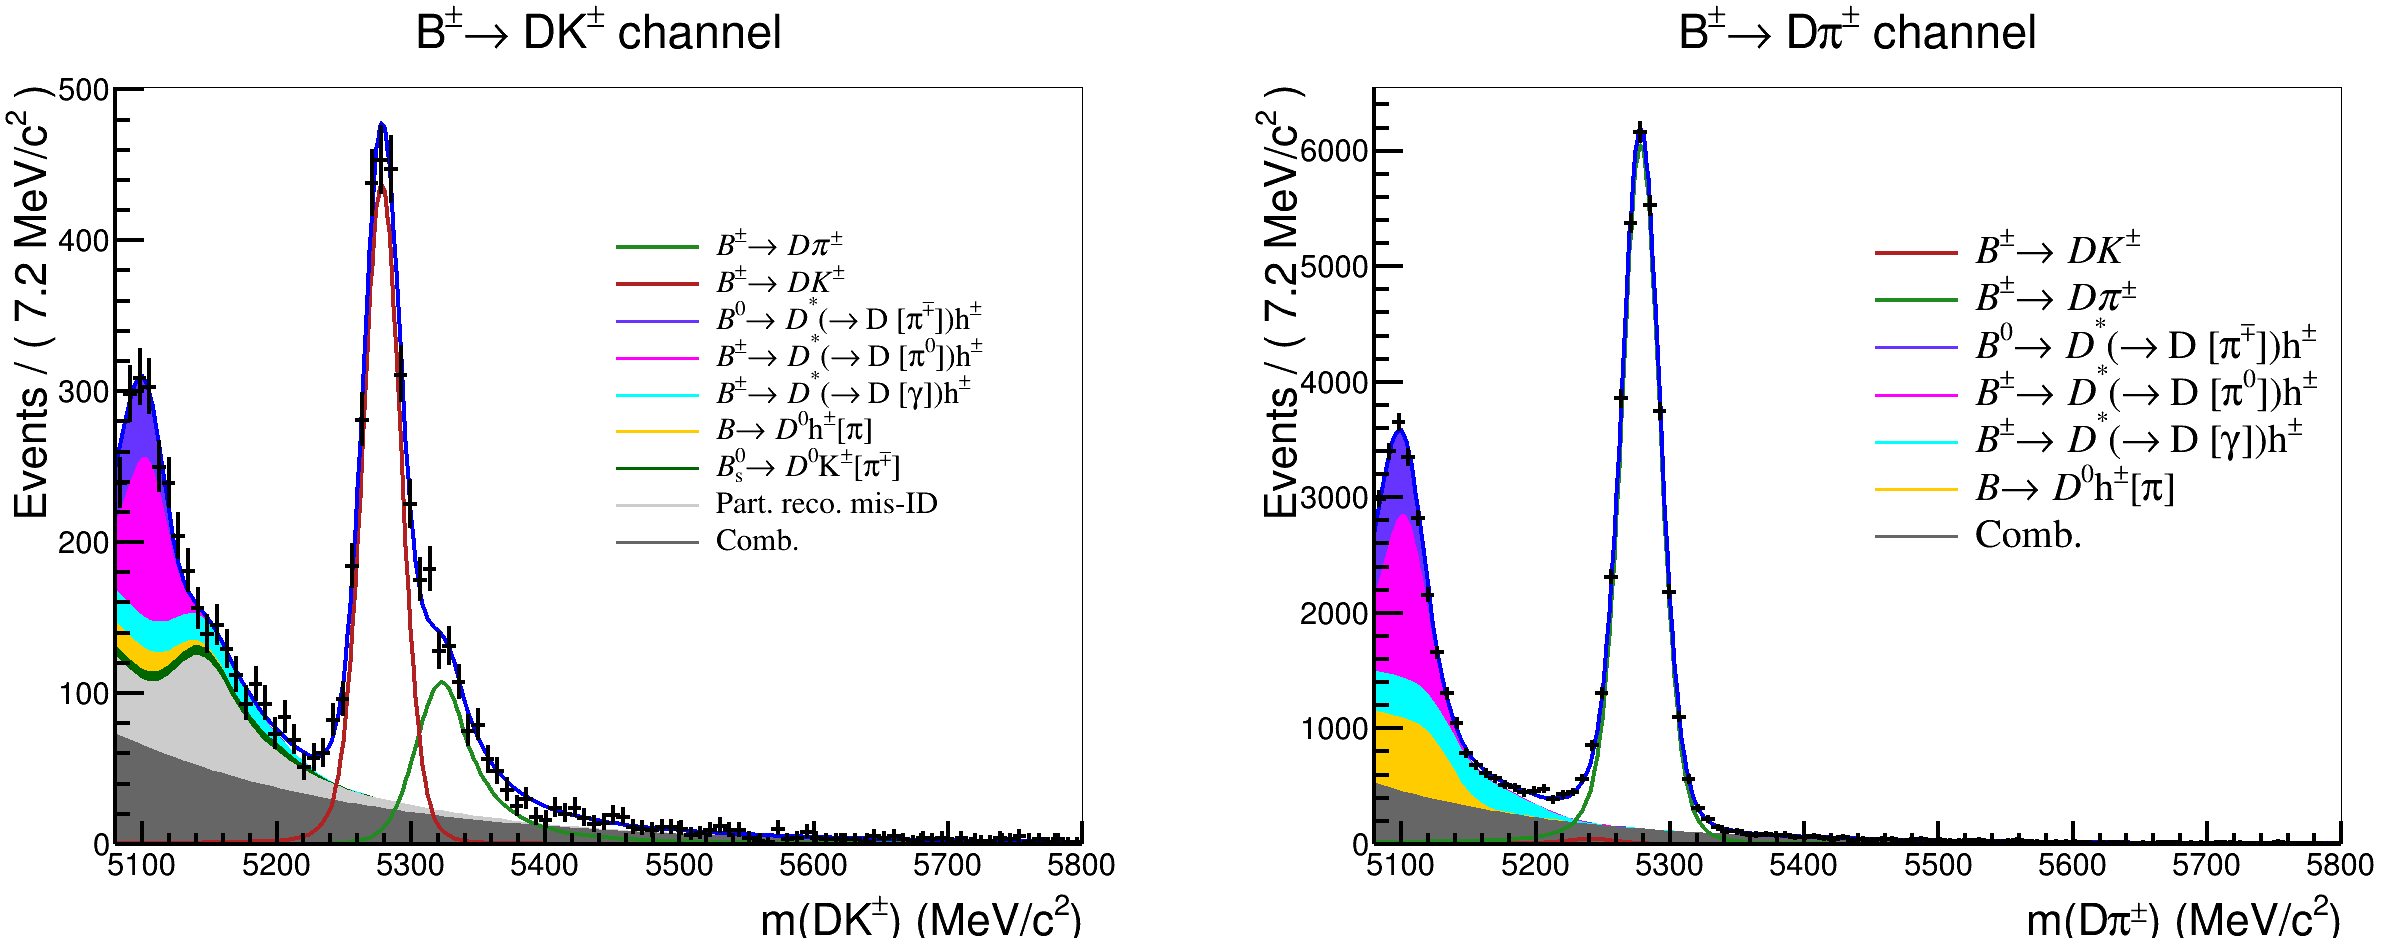
\includegraphics[width = 1.0\textwidth]{Plots/GlobalFit.png}
    \caption{Global fit of $B^\pm$ mass distribution for the $DK^\pm$ channel (left) and $D\pi^\pm$ channel (right)}
  \end{figure}
  \vspace{-0.5cm}
  \begin{itemize}
    \item{$B^\pm\to DK^\pm$ yield: $\SI{2290(59)}{}$}
    \item{$B^\pm\to D\pi^\pm$ yield: $\SI{33113(211)}{}$}
  \end{itemize}
\end{frame}

\begin{frame}{Global fit toy studies}
  \begin{itemize}
    \setlength\itemsep{1.2em}
    \item{Generated $1000$ toy datasets using the fitted parameters}
    \item{Almost all free parameters have pull distributions with zero mean and standard deviation $1$}
    \item{Consistent with LHCb-ANA-2020-001}
  \end{itemize}
\end{frame}

\begin{frame}{Global fit toy studies}
  \begin{figure}
    \centering
    \vspace{-0.2cm}
    \begin{subfigure}{0.33\textwidth}
      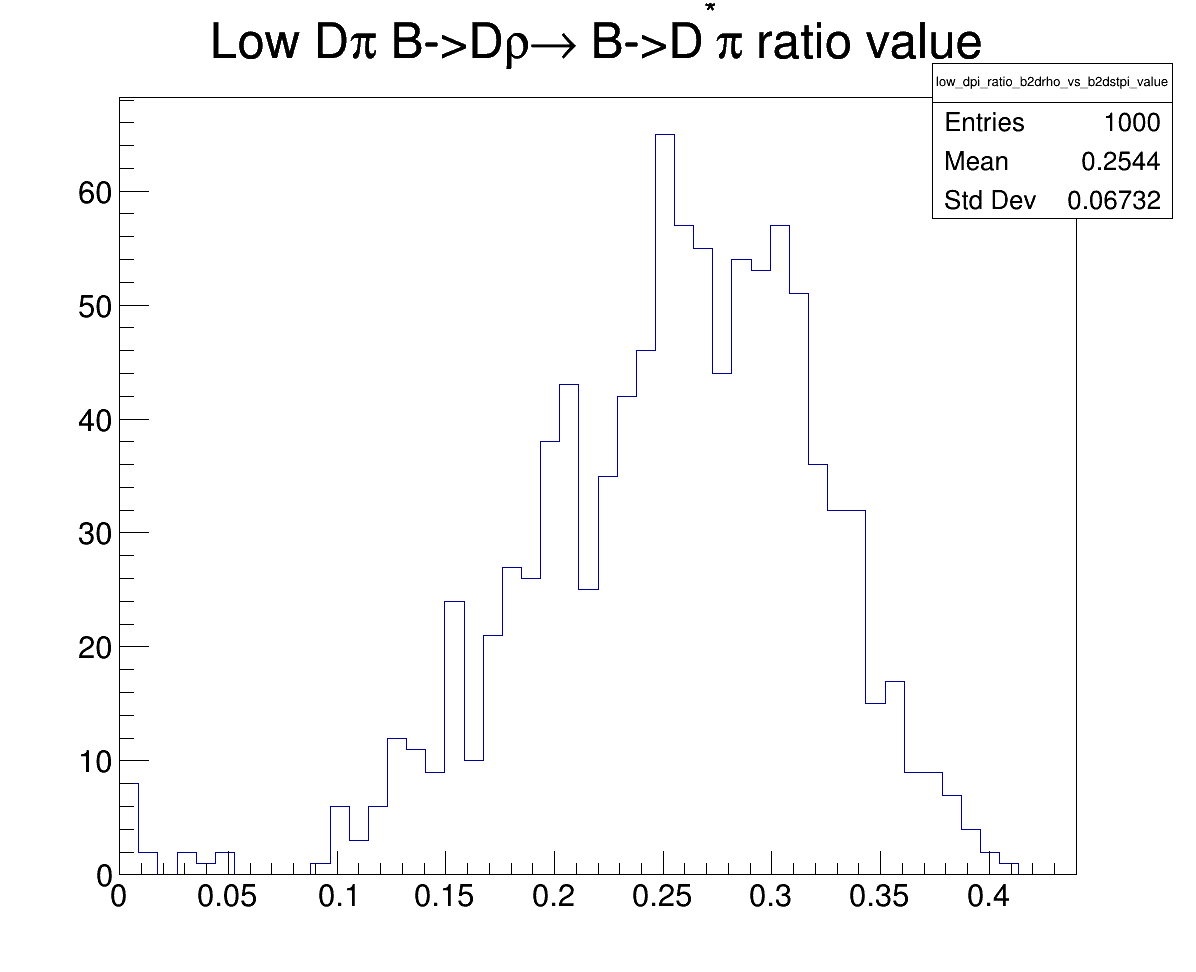
\includegraphics[width = 1.0\textwidth]{Plots/low_dpi_ratio_b2drho_vs_b2dstpi_value.png}
      \caption{Value}
    \end{subfigure}%
    \begin{subfigure}{0.33\textwidth}
      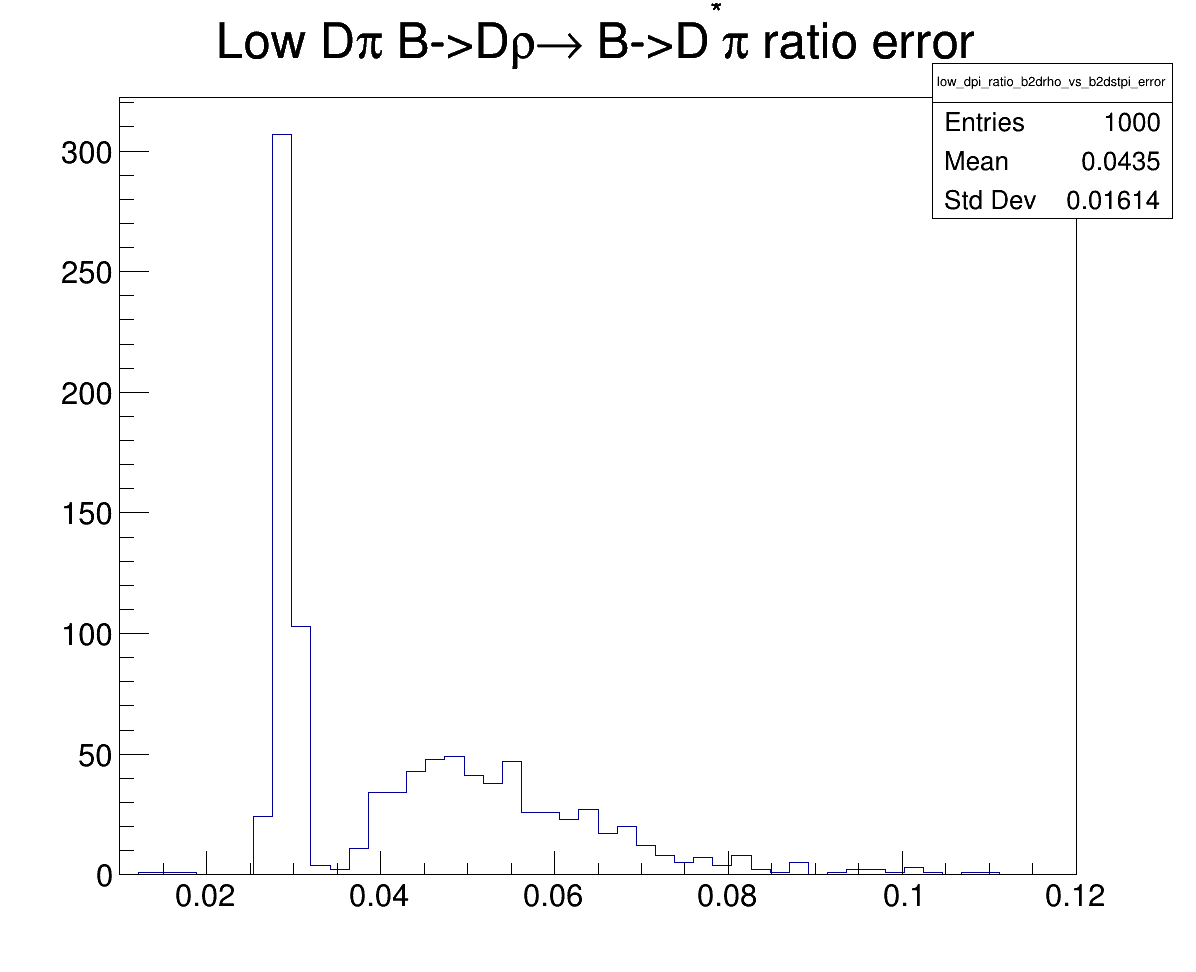
\includegraphics[width = 1.0\textwidth]{Plots/low_dpi_ratio_b2drho_vs_b2dstpi_error.png}
      \caption{Error}
    \end{subfigure}%
    \begin{subfigure}{0.33\textwidth}
      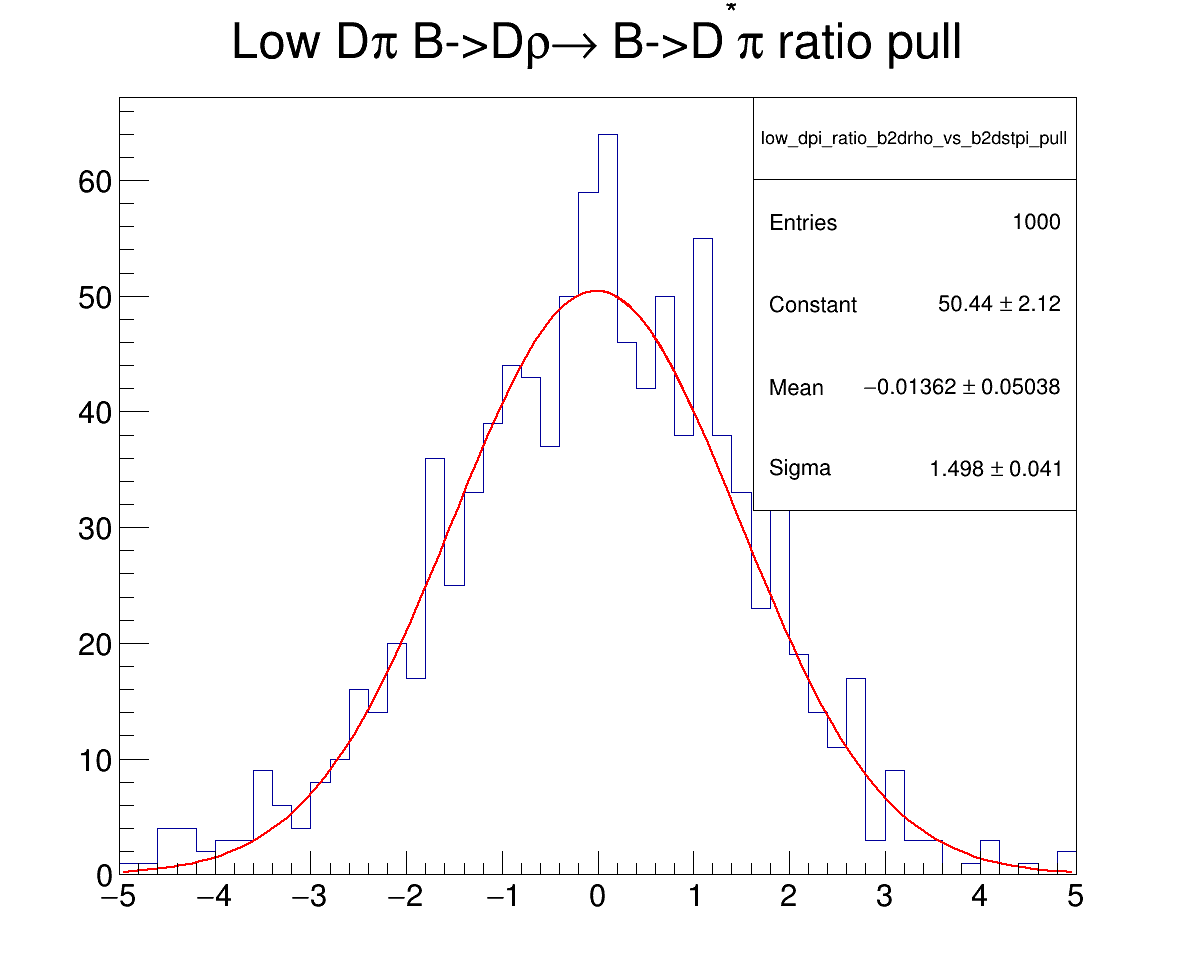
\includegraphics[width = 1.0\textwidth]{Plots/low_dpi_ratio_b2drho_vs_b2dstpi_pull.png}
      \caption{Pull}
    \end{subfigure}
    \caption{\texttt{low\_dpi\_ratio\_b2drho\_vs\_b2dstpi}}
  \end{figure}
\end{frame}

\begin{frame}{Global fit toy studies}
  \begin{figure}
    \centering
    \vspace{-0.2cm}
    \begin{subfigure}{0.33\textwidth}
      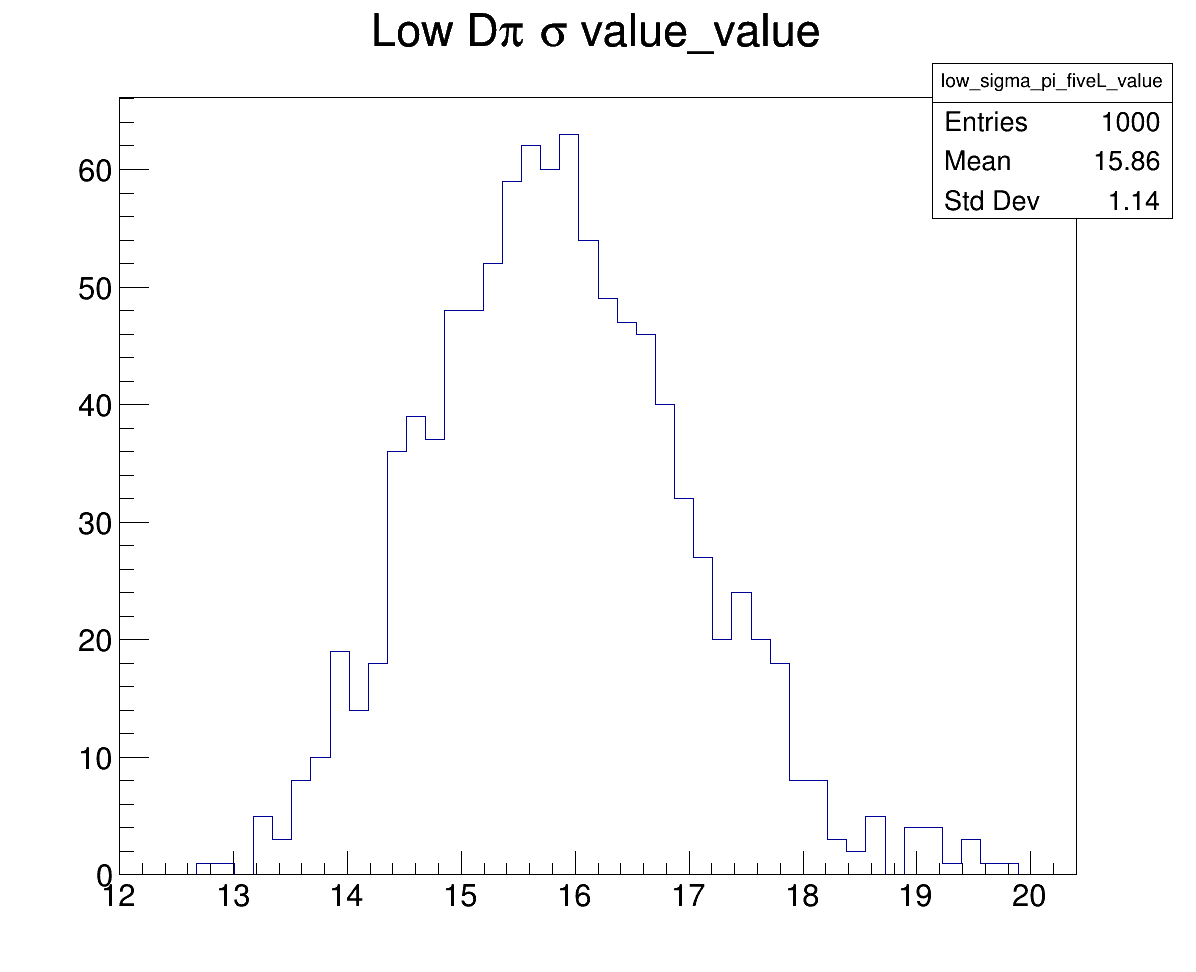
\includegraphics[width = 1.0\textwidth]{Plots/low_sigma_pi_fiveL_value.png}
      \caption{Value}
    \end{subfigure}%
    \begin{subfigure}{0.33\textwidth}
      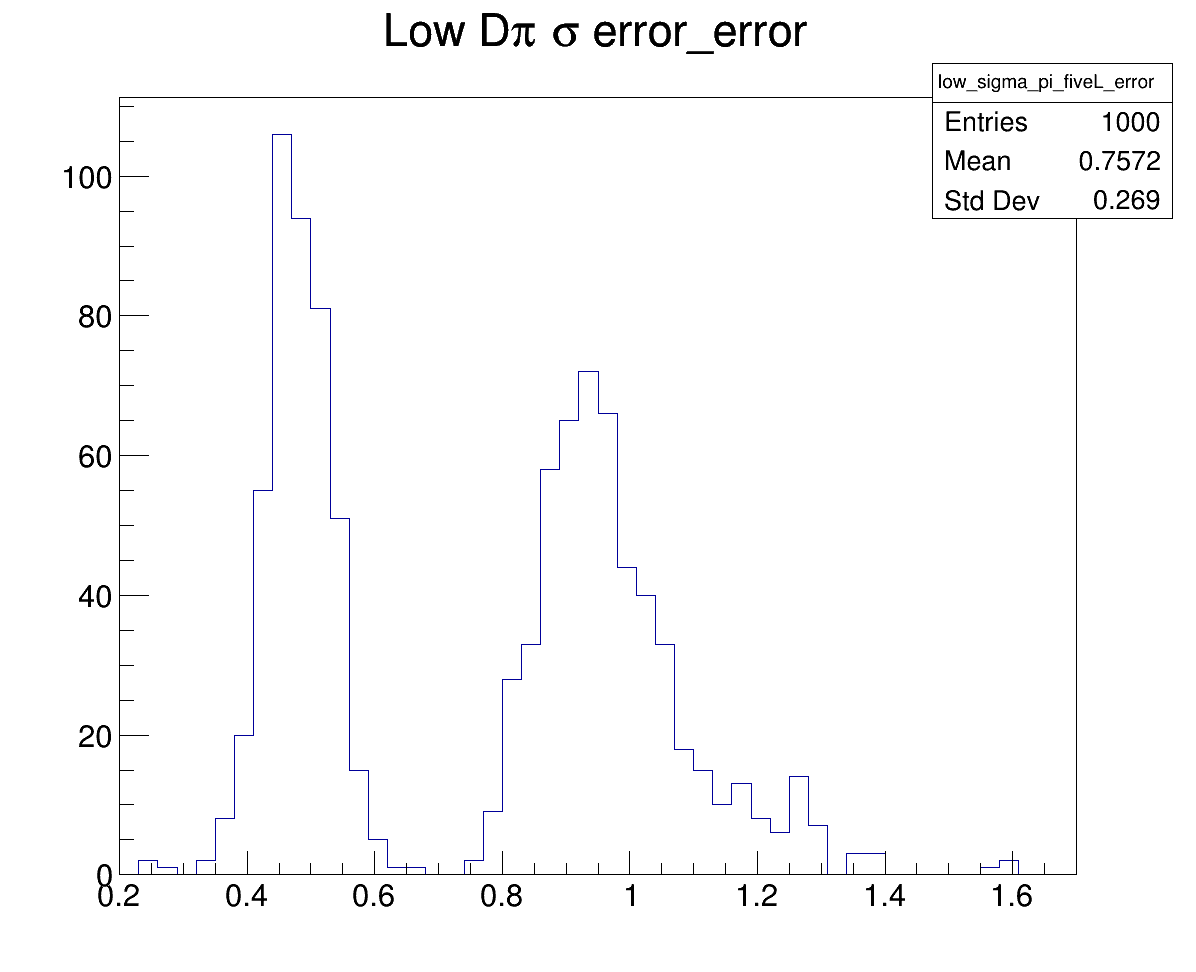
\includegraphics[width = 1.0\textwidth]{Plots/low_sigma_pi_fiveL_error.png}
      \caption{Error}
    \end{subfigure}%
    \begin{subfigure}{0.33\textwidth}
      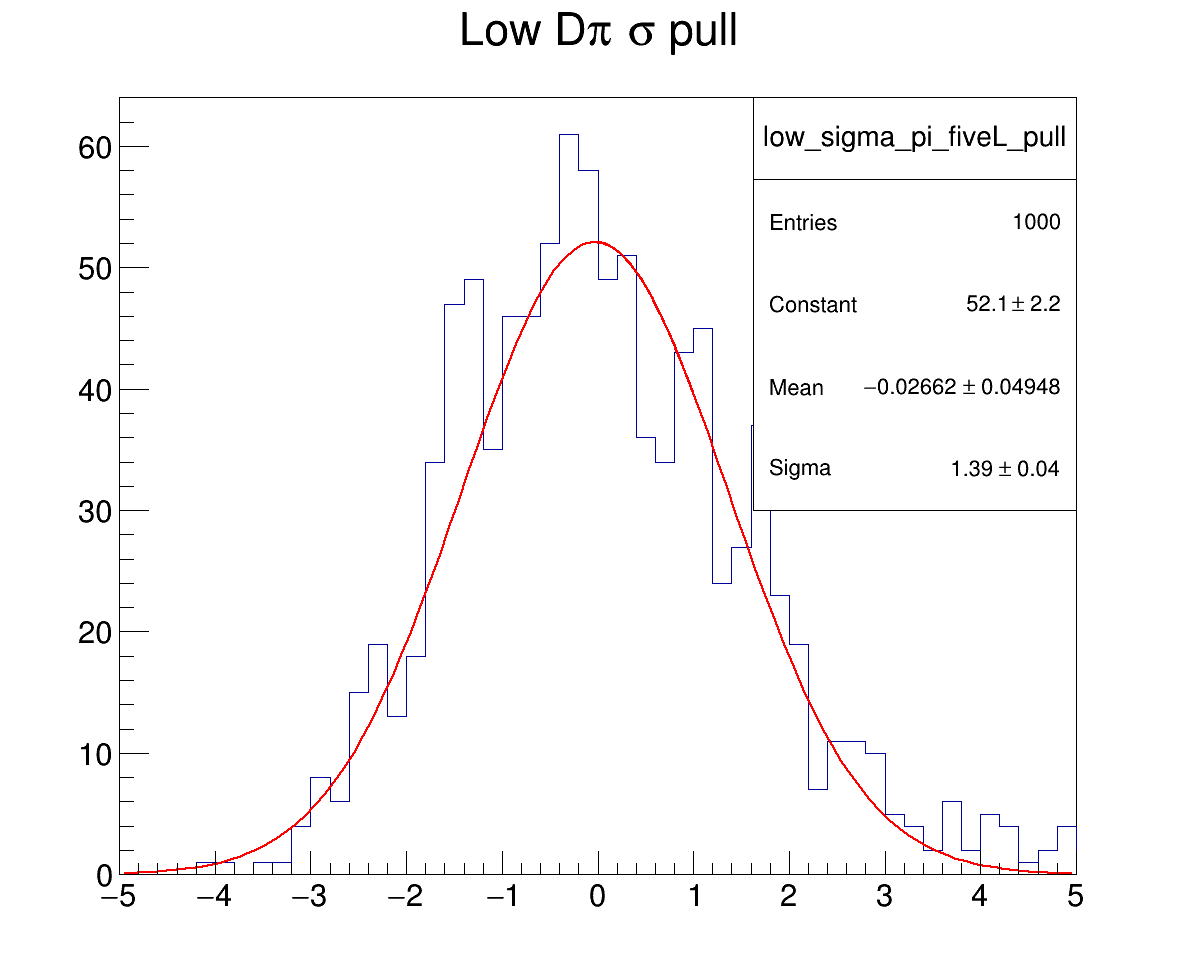
\includegraphics[width = 1.0\textwidth]{Plots/low_sigma_pi_fiveL_pull.png}
      \caption{Pull}
    \end{subfigure}
    \caption{\texttt{low\_sigma\_pi\_fiveL\_error.png}}
  \end{figure}
\end{frame}

\section{Binned CP fit}
\begin{frame}{Binned CP fit}
  \begin{center}
    {\huge Binned CP fit}
  \end{center}
\end{frame}

\begin{frame}{Binned CP fit}
  \begin{itemize}
    \setlength\itemsep{1.2em}
    \item{Use $8$ bins for now}
    \item{$c_i$ and $s_i$ calculated using MC integration of LHCb amplitude model}
    \item{Fit for CP observables}
    \item{PDF shape parameters fixed from global fit}
    \item{Yield of signal, low mass partially reconstructed background and combinatorial background floated}
    \item{Fractional yields $K_i$ ($F_i$) floated}
  \end{itemize}
  \begin{equation*}
    \mathcal{R}_i = 
    \begin{cases}
      F_i, \quad i = -8 \\
      F_i/\sum_{j\geq i}, -8 < i\leq+8
    \end{cases}
  \end{equation*}
\end{frame}

\begin{frame}{Fitted CP observables}
  \begin{figure}
    \centering
    \vspace{-0.2cm}
    \begin{subfigure}{0.5\textwidth}
      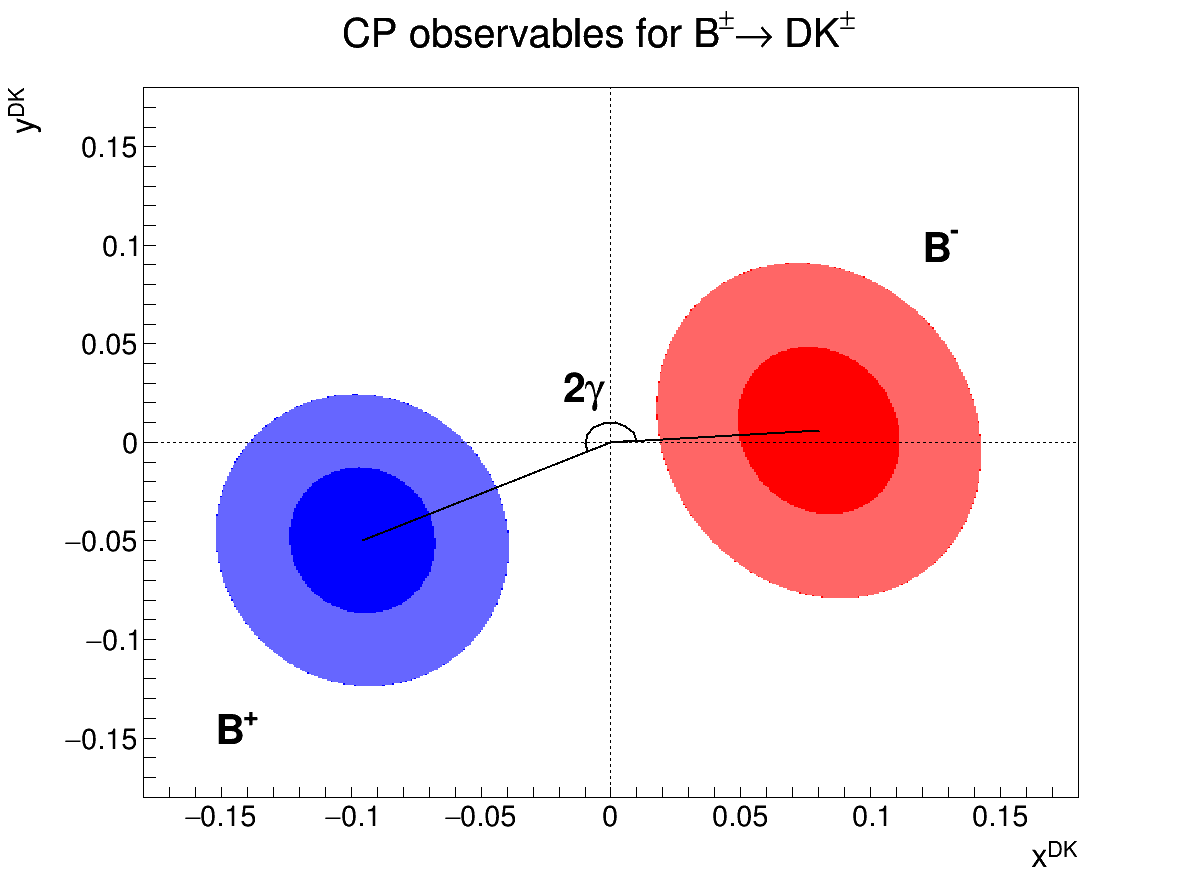
\includegraphics[width = 1.0\textwidth]{Plots/CPContours.png}
      \caption{$x_\pm^{DK}$ and $y_\pm^{DK}$}
    \end{subfigure}%
    \begin{subfigure}{0.5\textwidth}
      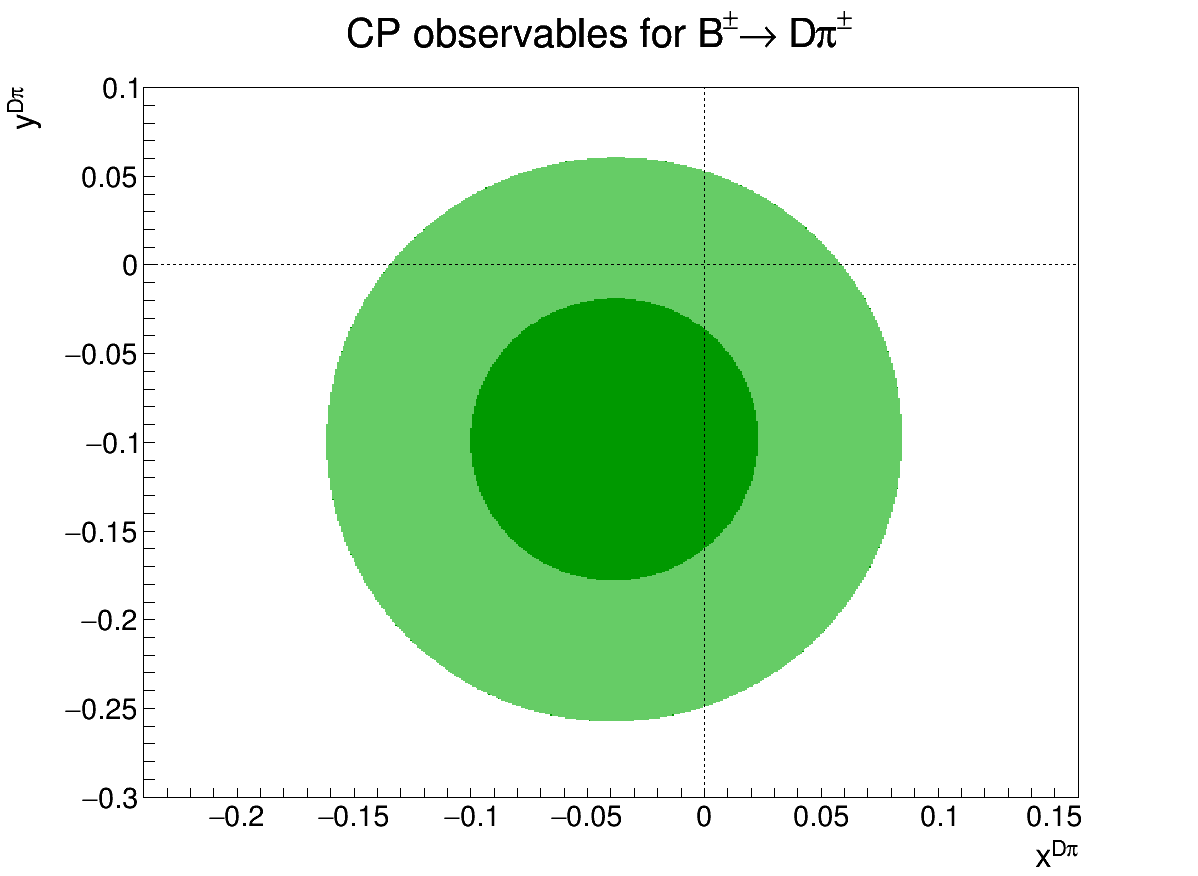
\includegraphics[width = 1.0\textwidth]{Plots/CPXiContours.png}
      \caption{$x_\xi^{D\pi}$ and $y_\xi^{D\pi}$}
    \end{subfigure}
    \caption{$68.2\%$ and $95.5\%$ confidence intervals of CP observables}
  \end{figure}
\end{frame}

\begin{frame}{CP fit toy studies}
  \begin{figure}
    \centering
    \begin{subfigure}{0.25\textwidth}
      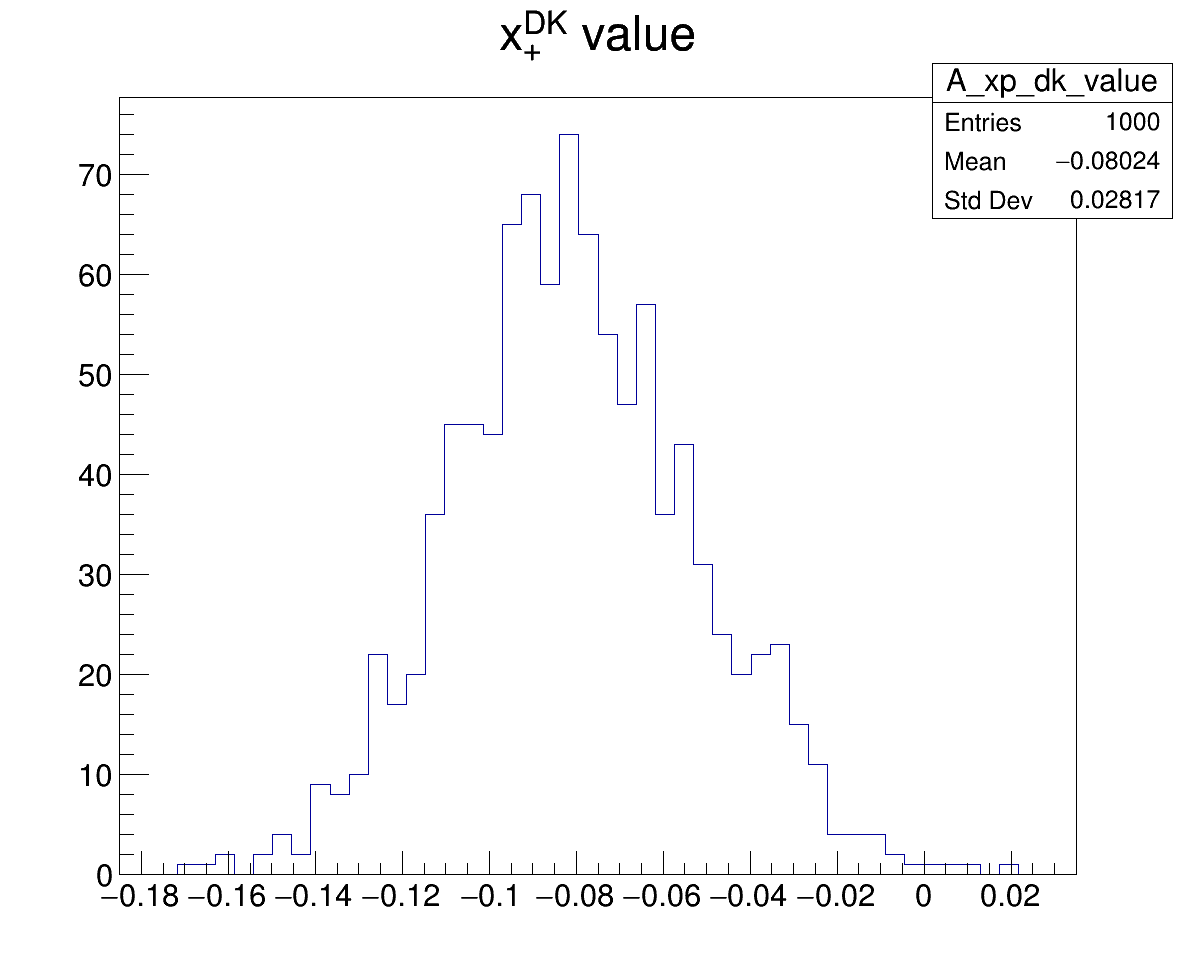
\includegraphics[width = 1.0\textwidth]{Plots/A_xp_dk_value.png}
      \caption{Value}
    \end{subfigure}%
    \begin{subfigure}{0.25\textwidth}
      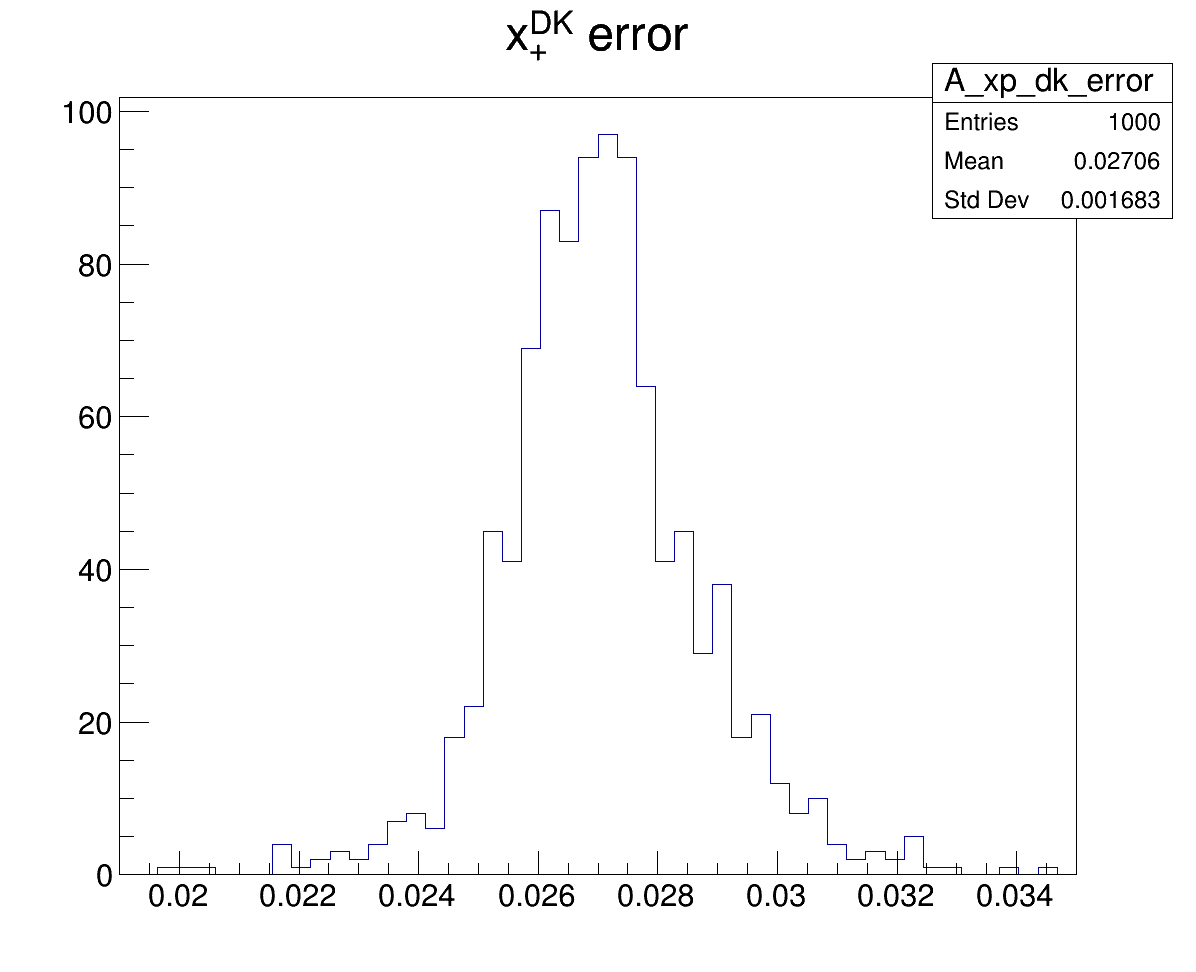
\includegraphics[width = 1.0\textwidth]{Plots/A_xp_dk_error.png}
      \caption{Error}
    \end{subfigure}%
    \begin{subfigure}{0.25\textwidth}
      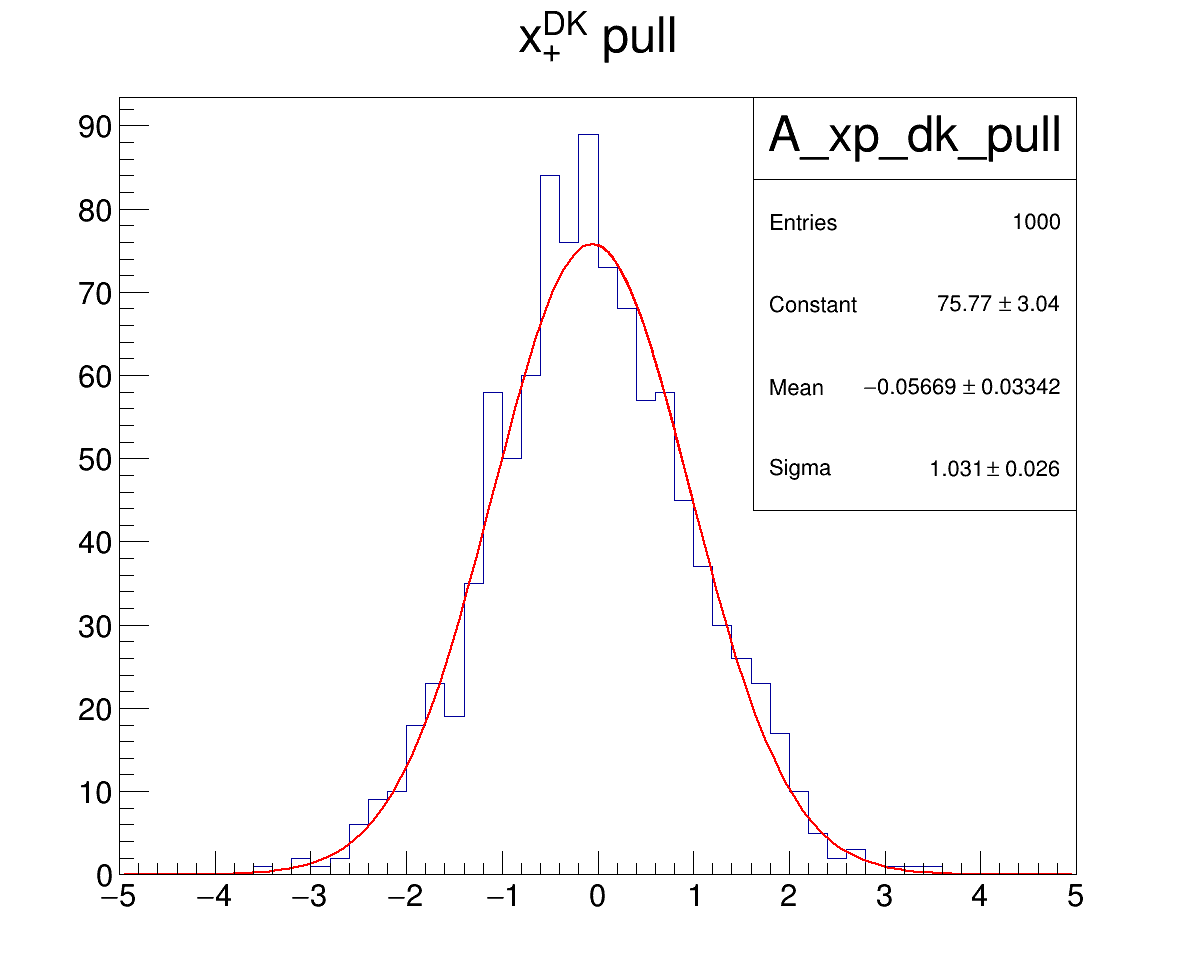
\includegraphics[width = 1.0\textwidth]{Plots/A_xp_dk_pull.png}
      \caption{Pull}
    \end{subfigure}
    \caption{$x_+^{DK}$}
  \end{figure}
  \begin{figure}
    \centering
    \vspace{-0.15cm}
    \begin{subfigure}{0.25\textwidth}
      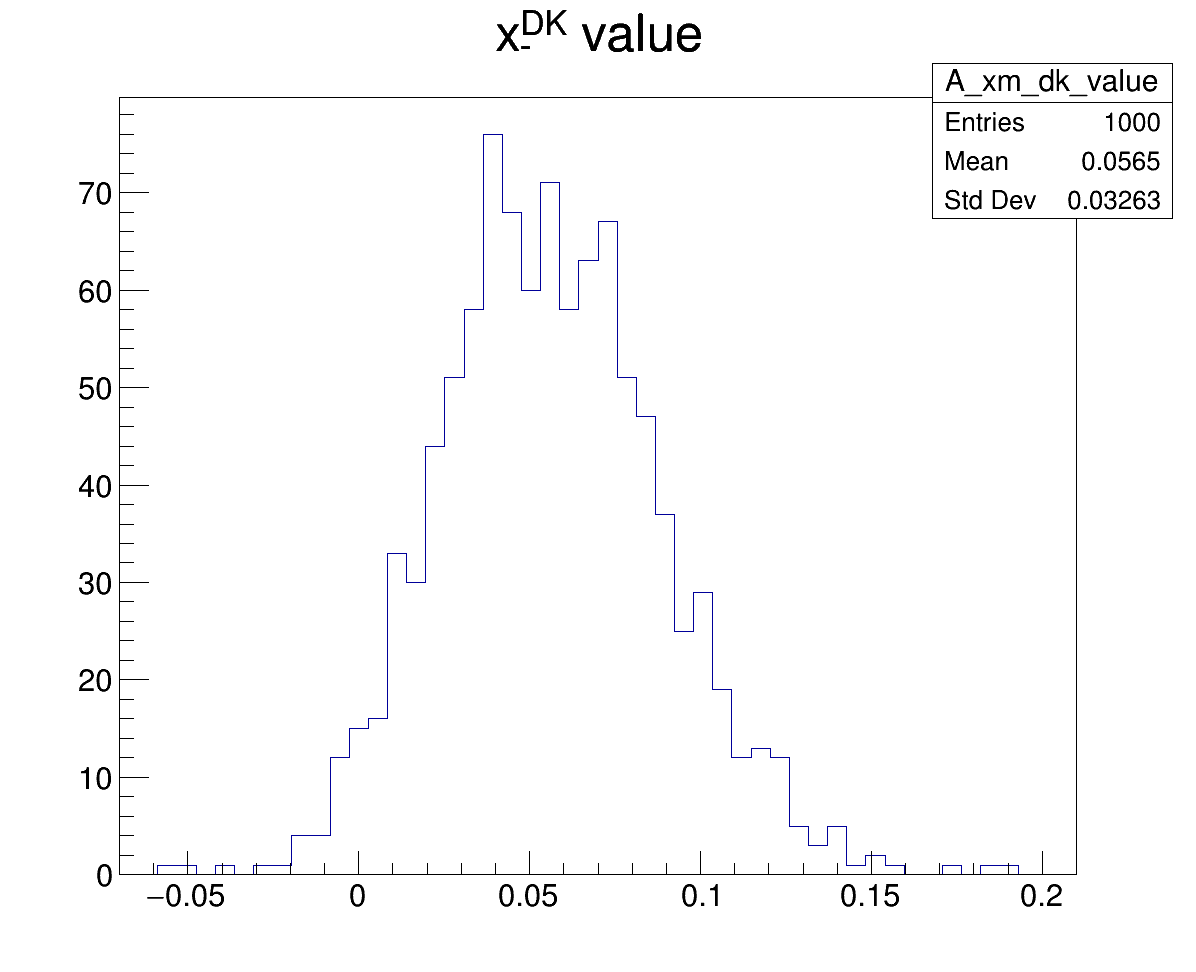
\includegraphics[width = 1.0\textwidth]{Plots/A_xm_dk_value.png}
      \caption{Value}
    \end{subfigure}%
    \begin{subfigure}{0.25\textwidth}
      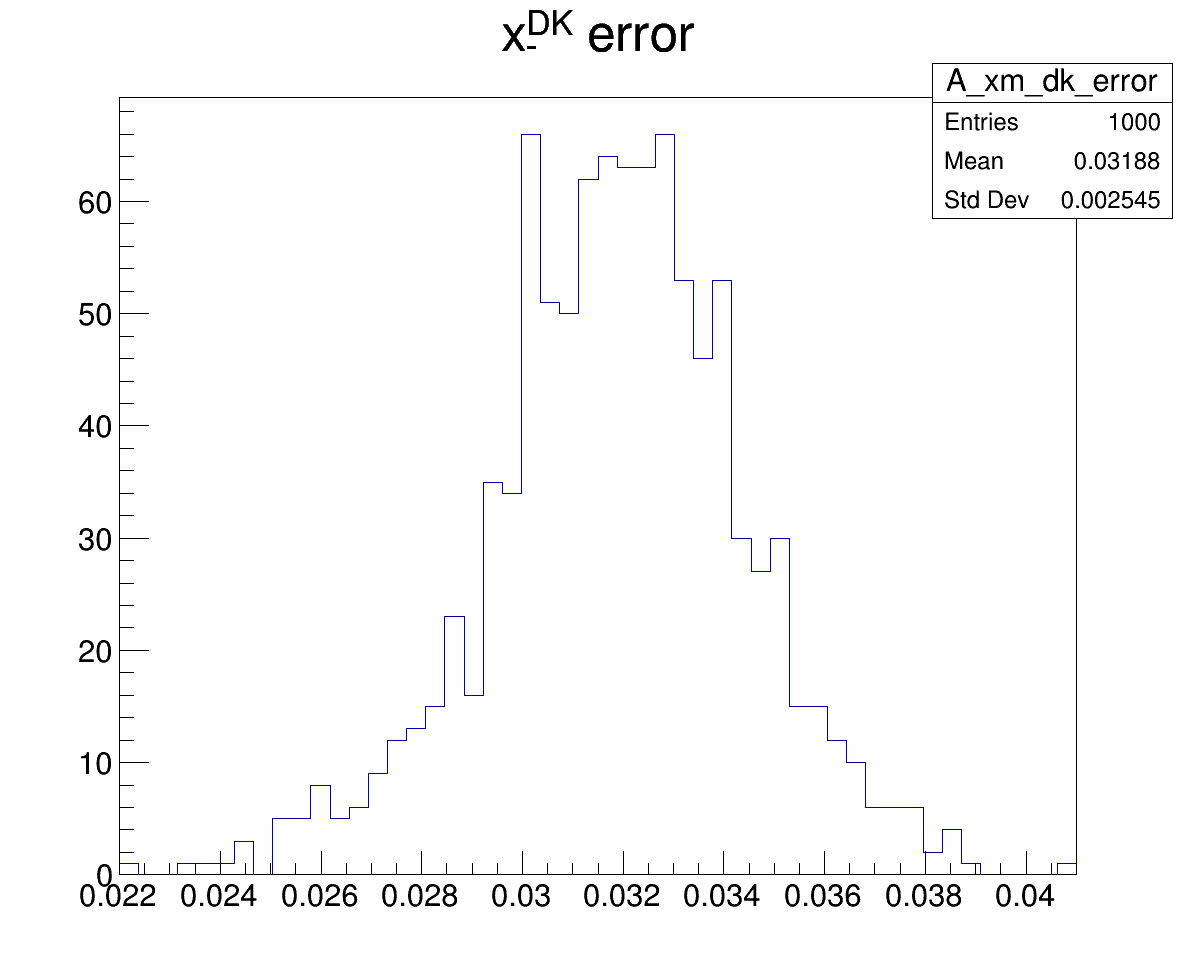
\includegraphics[width = 1.0\textwidth]{Plots/A_xm_dk_error.png}
      \caption{Error}
    \end{subfigure}%
    \begin{subfigure}{0.25\textwidth}
      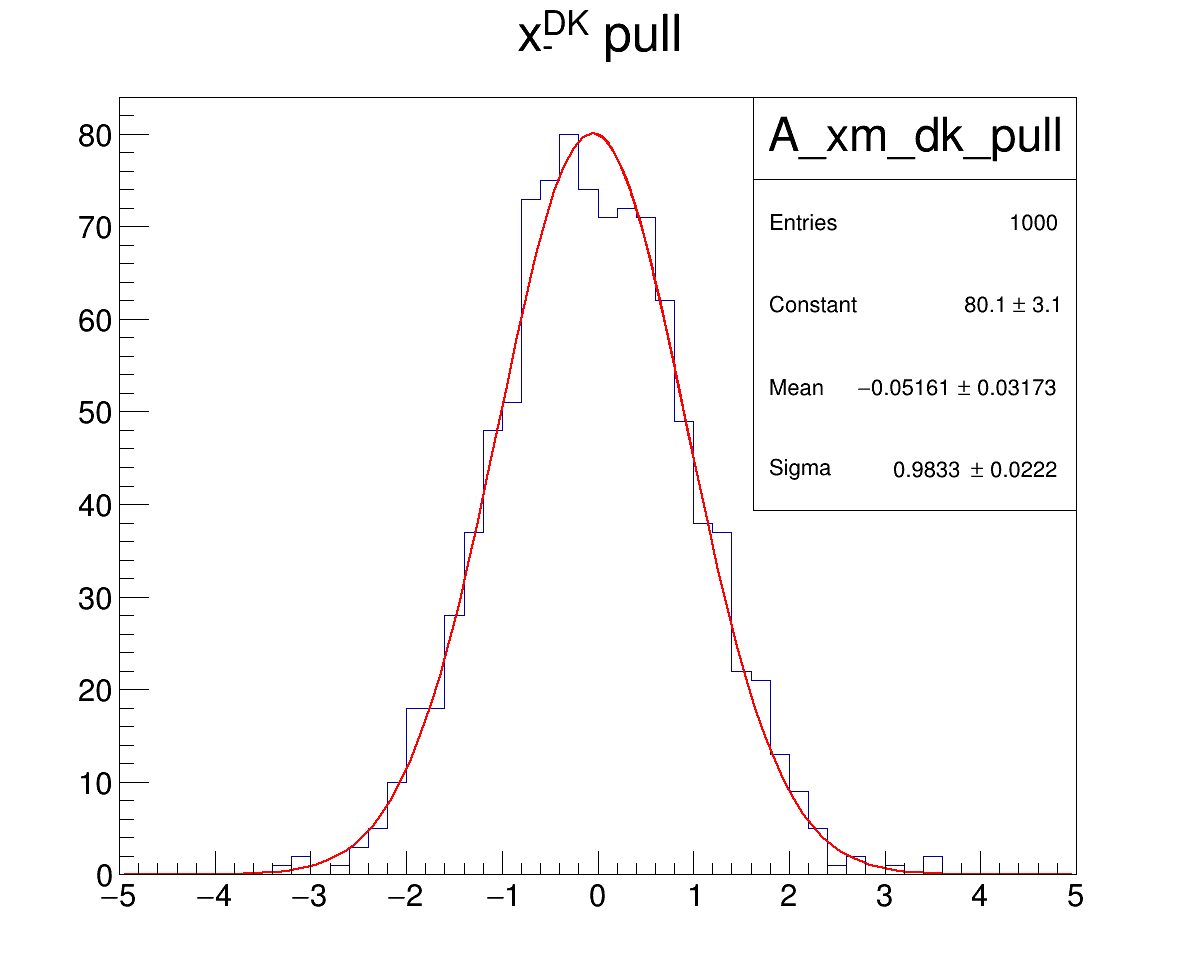
\includegraphics[width = 1.0\textwidth]{Plots/A_xm_dk_pull.png}
      \caption{Pull}
    \end{subfigure}
    \caption{$x_-^{DK}$}
  \end{figure}
\end{frame}

\begin{frame}{CP fit toy studies}
  \begin{figure}
    \centering
    \begin{subfigure}{0.25\textwidth}
      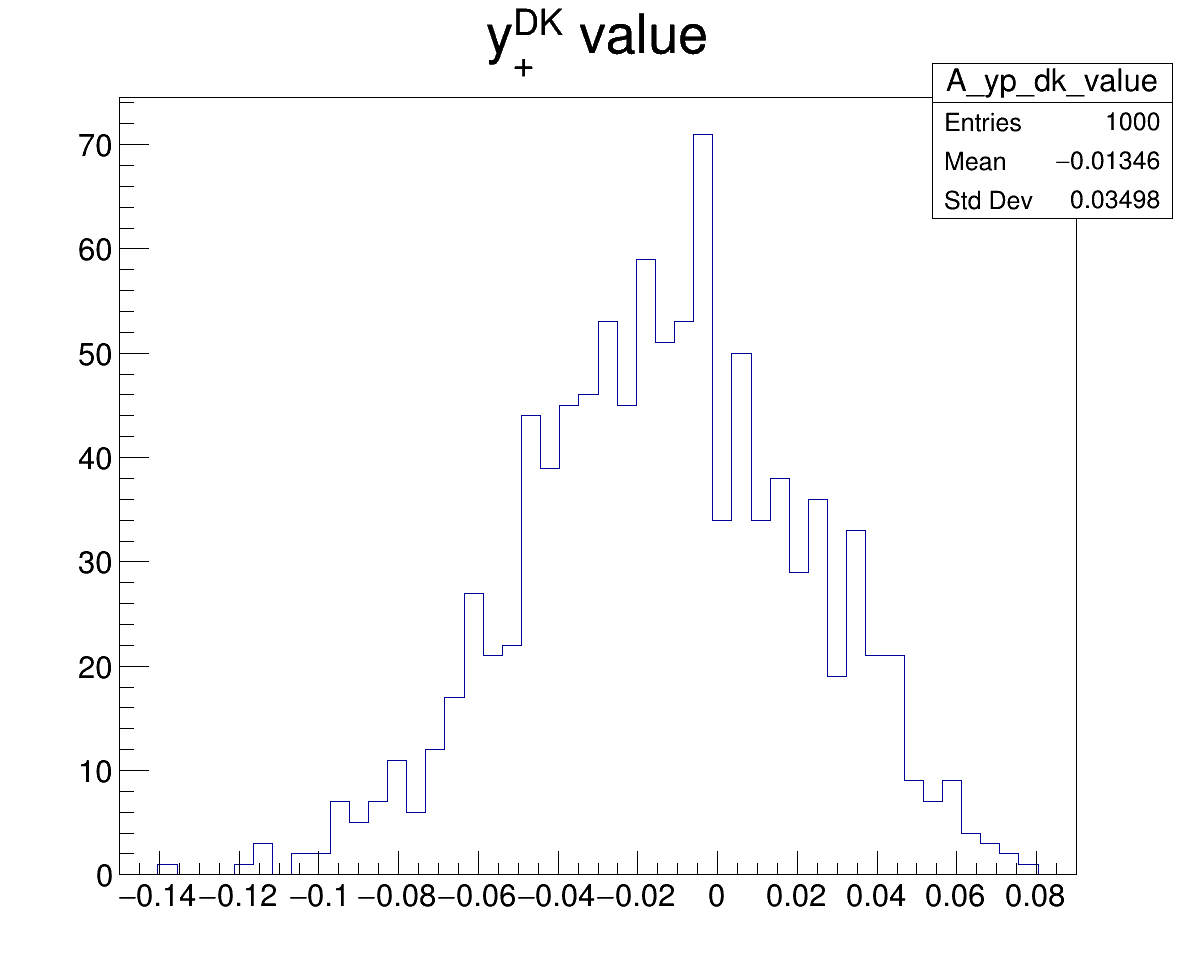
\includegraphics[width = 1.0\textwidth]{Plots/A_yp_dk_value.png}
      \caption{Value}
    \end{subfigure}%
    \begin{subfigure}{0.25\textwidth}
      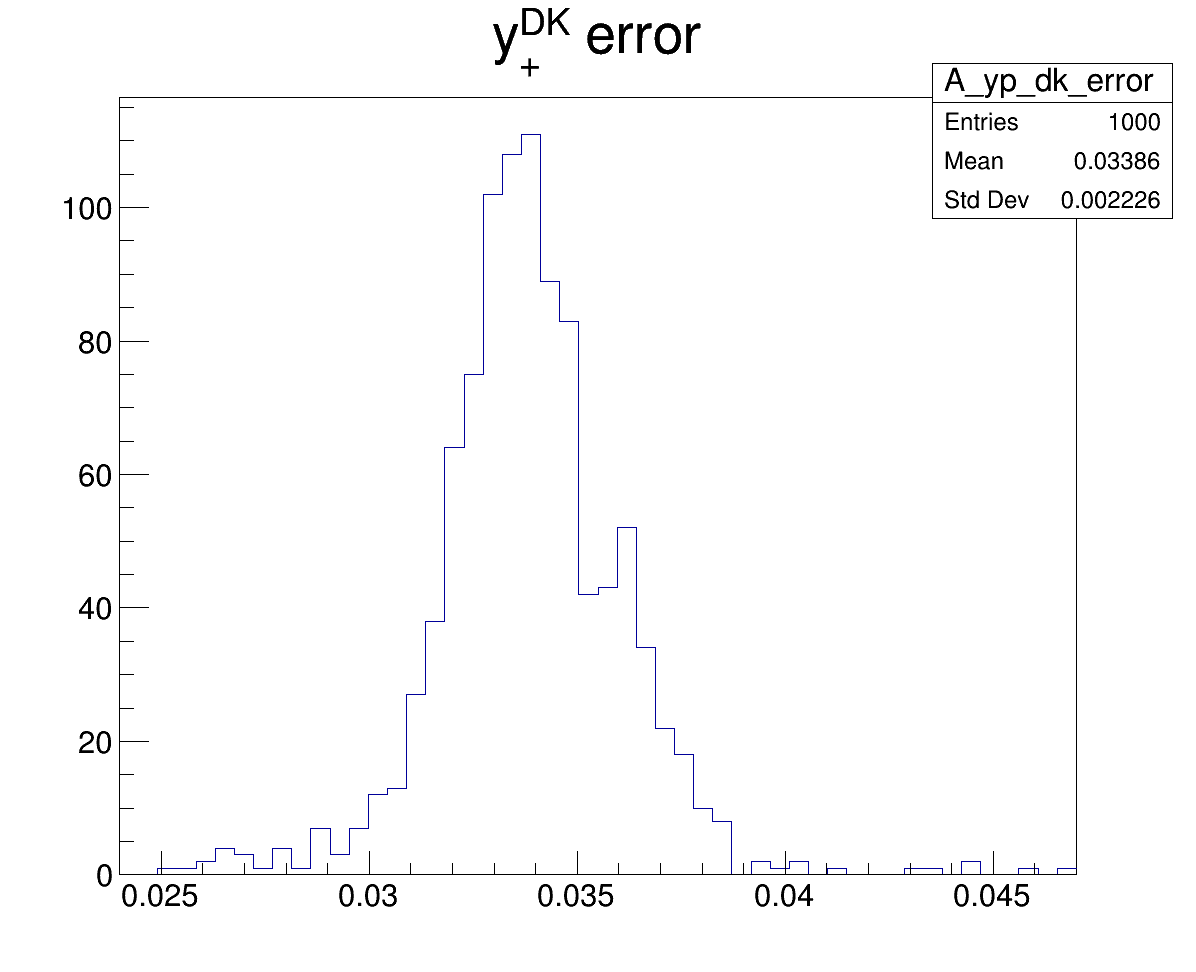
\includegraphics[width = 1.0\textwidth]{Plots/A_yp_dk_error.png}
      \caption{Error}
    \end{subfigure}%
    \begin{subfigure}{0.25\textwidth}
      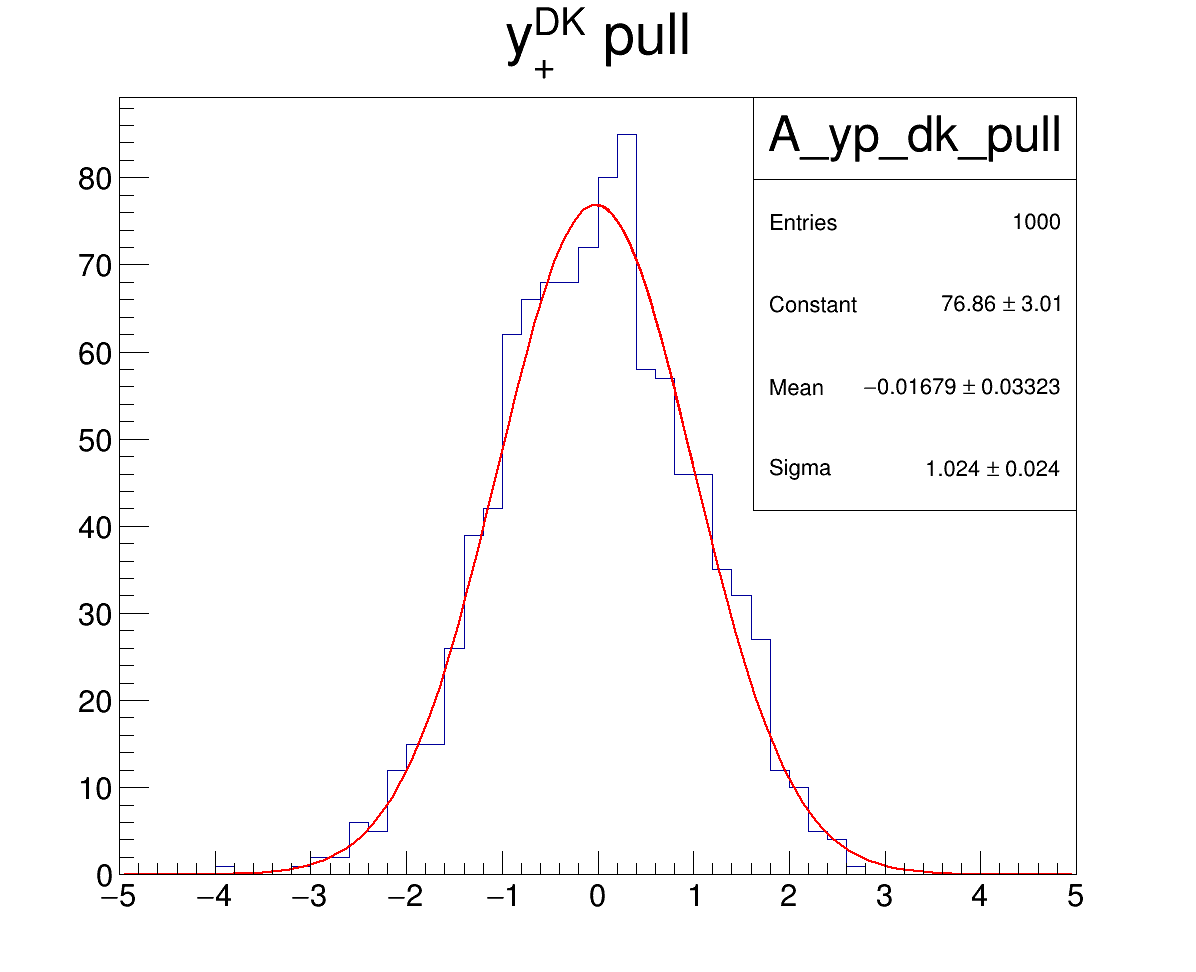
\includegraphics[width = 1.0\textwidth]{Plots/A_yp_dk_pull.png}
      \caption{Pull}
    \end{subfigure}
    \caption{$y_+^{DK}$}
  \end{figure}
  \begin{figure}
    \centering
    \vspace{-0.15cm}
    \begin{subfigure}{0.25\textwidth}
      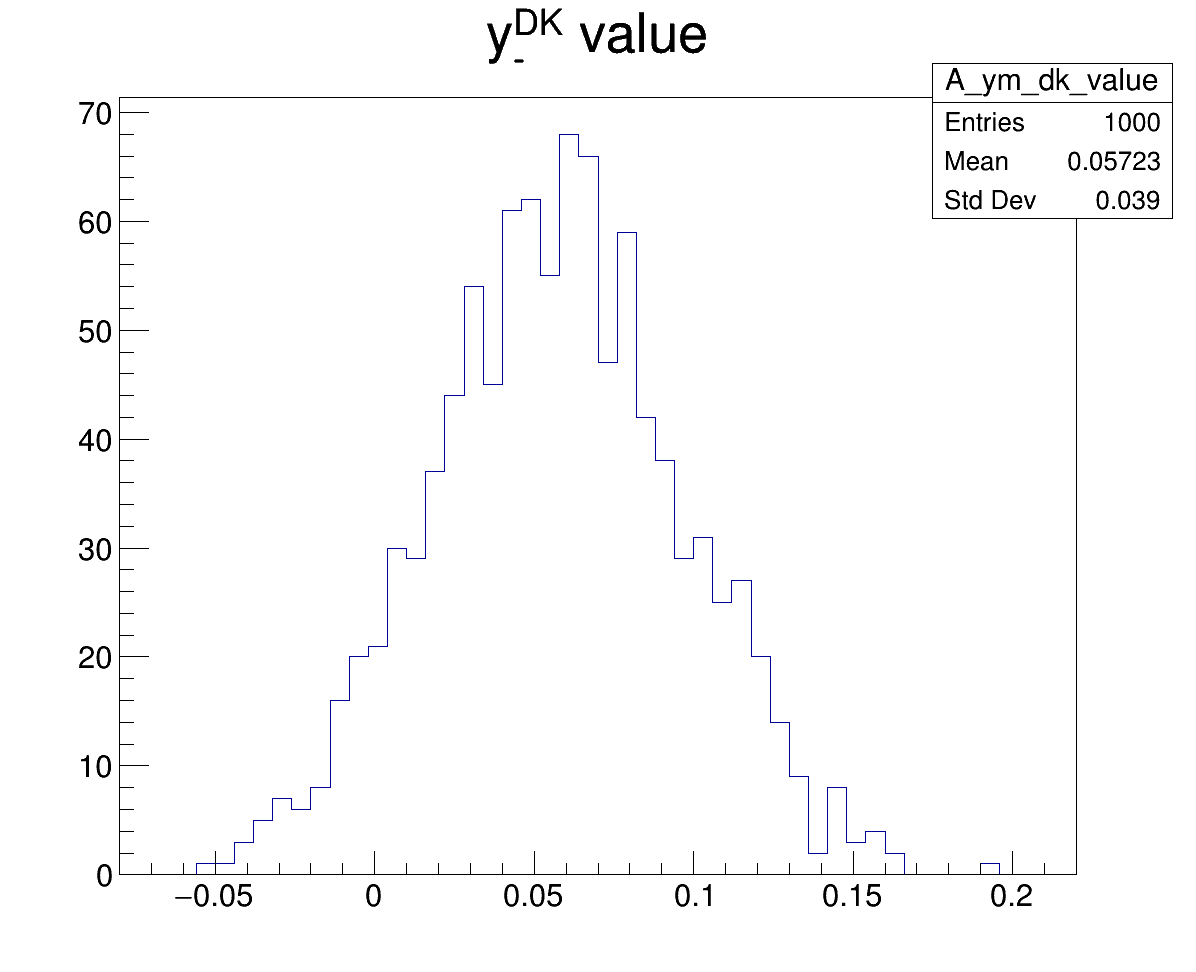
\includegraphics[width = 1.0\textwidth]{Plots/A_ym_dk_value.png}
      \caption{Value}
    \end{subfigure}%
    \begin{subfigure}{0.25\textwidth}
      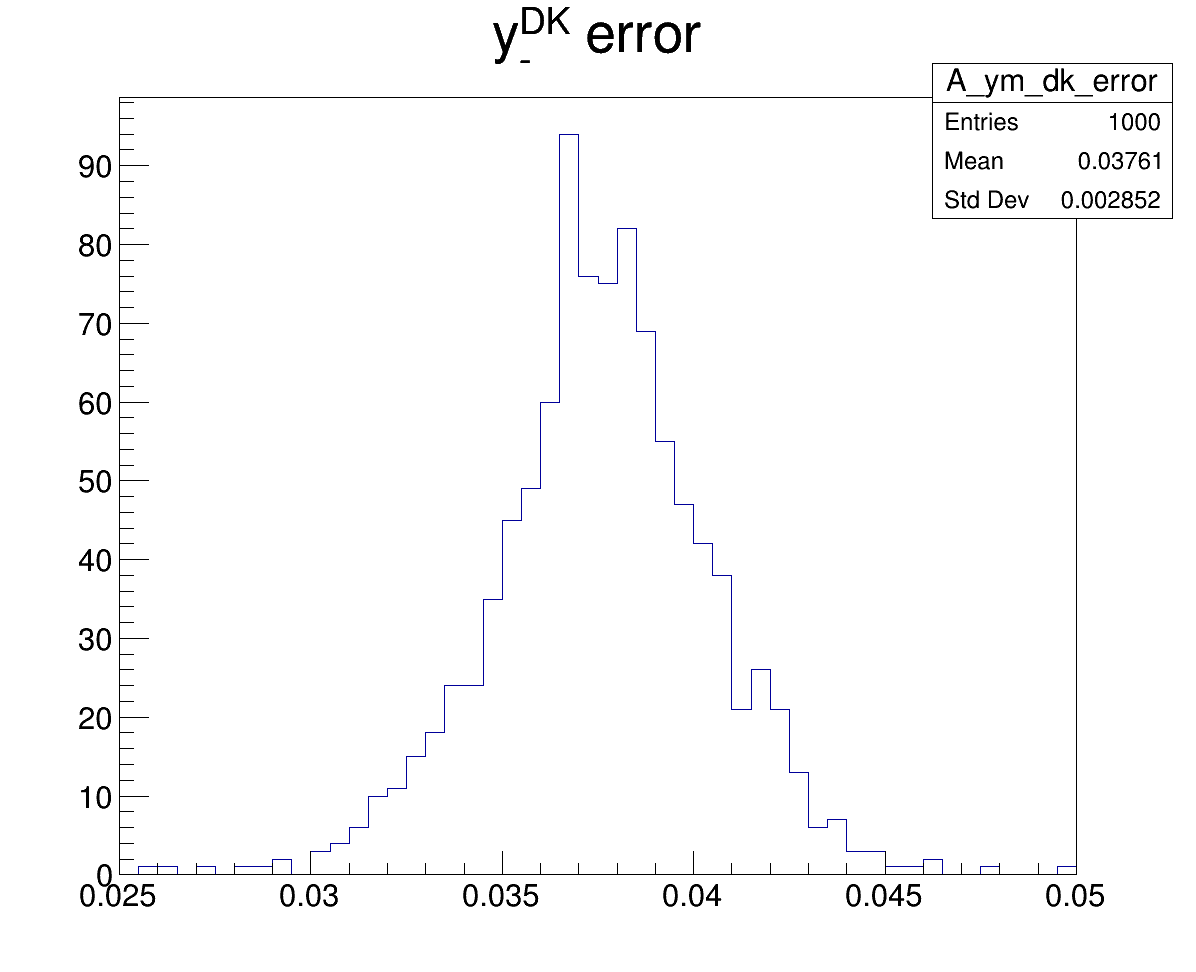
\includegraphics[width = 1.0\textwidth]{Plots/A_ym_dk_error.png}
      \caption{Error}
    \end{subfigure}%
    \begin{subfigure}{0.25\textwidth}
      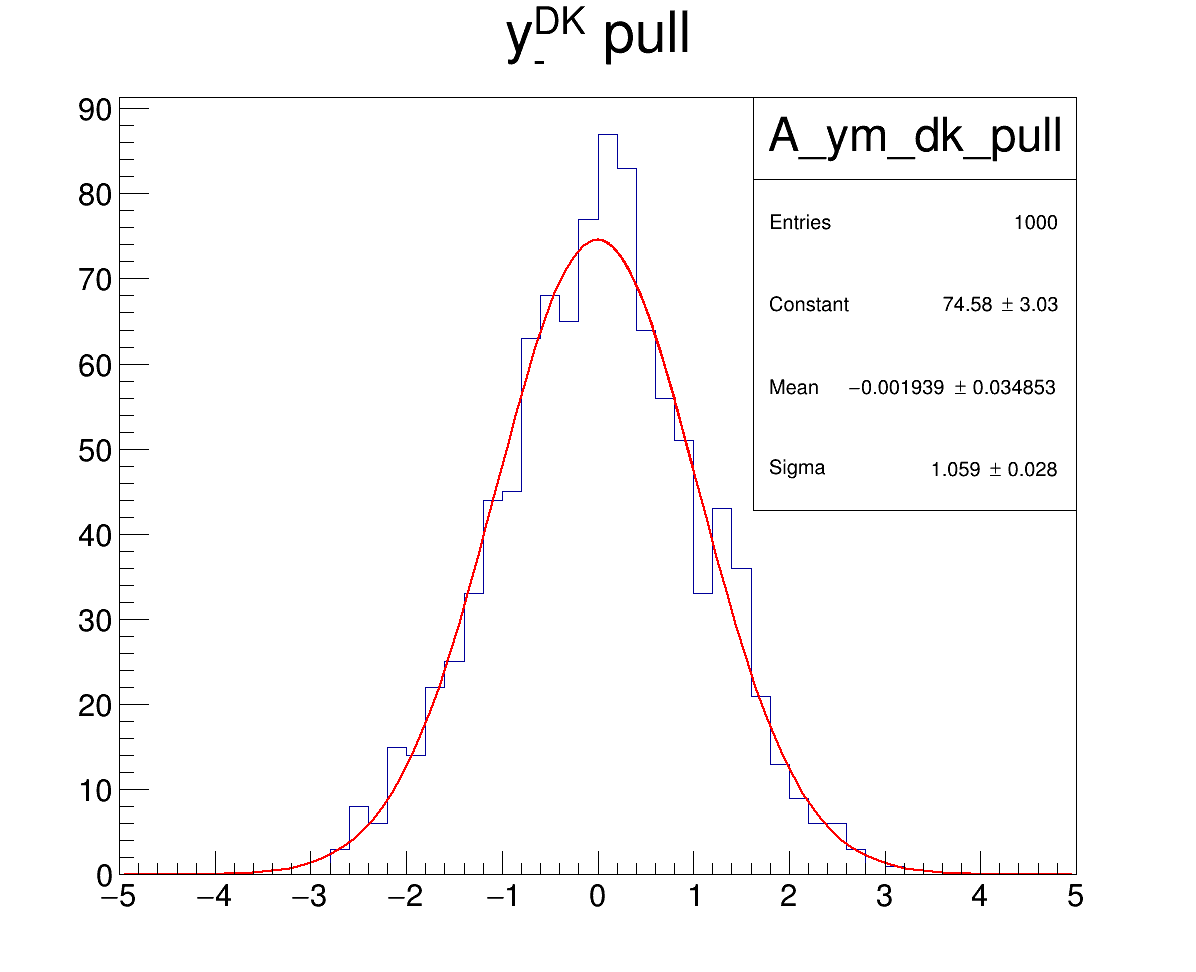
\includegraphics[width = 1.0\textwidth]{Plots/A_ym_dk_pull.png}
      \caption{Pull}
    \end{subfigure}
    \caption{$y_-^{DK}$}
  \end{figure}
\end{frame}

\begin{frame}{CP fit toy studies}
  \begin{figure}
    \centering
    \begin{subfigure}{0.25\textwidth}
      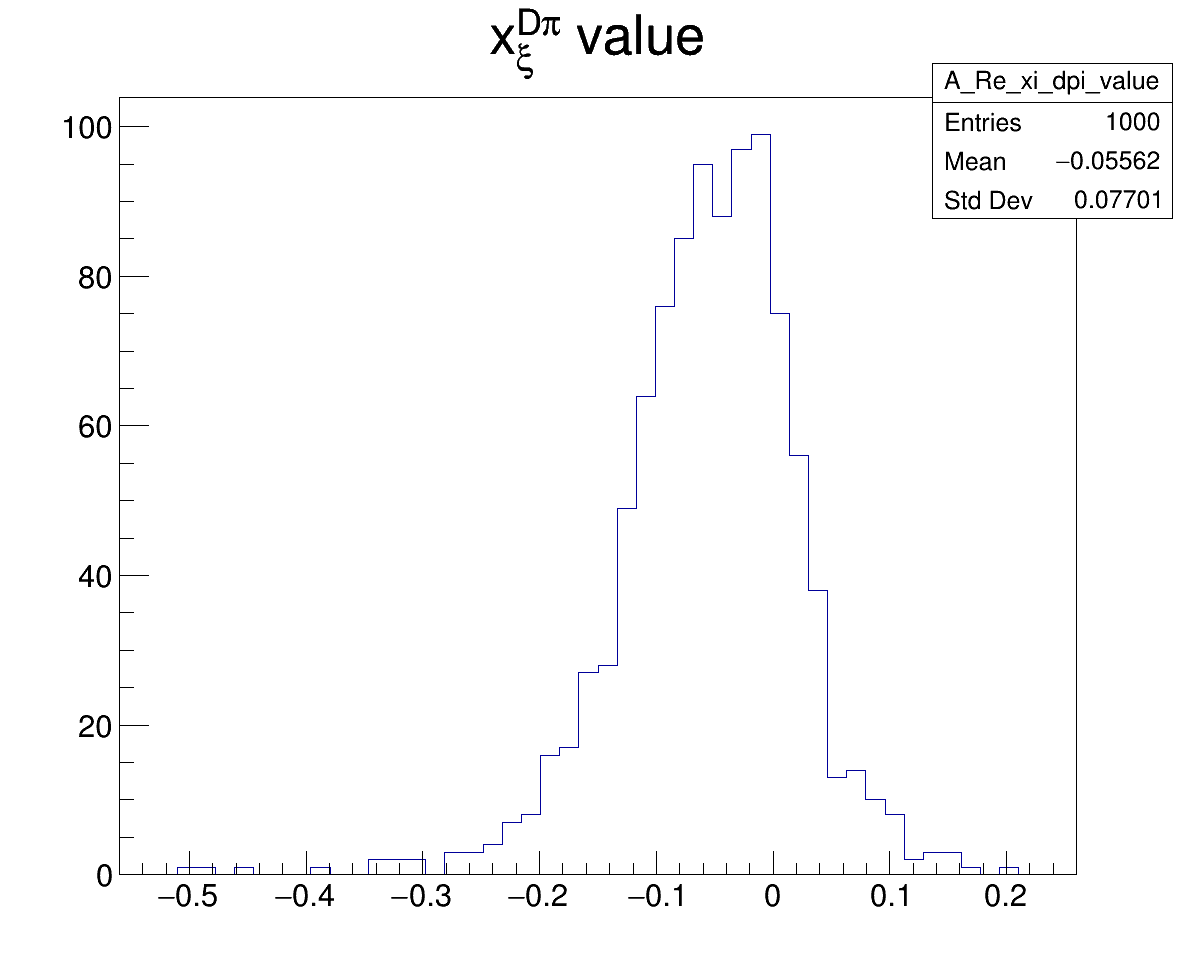
\includegraphics[width = 1.0\textwidth]{Plots/A_Re_xi_dpi_value.png}
      \caption{Value}
    \end{subfigure}%
    \begin{subfigure}{0.25\textwidth}
      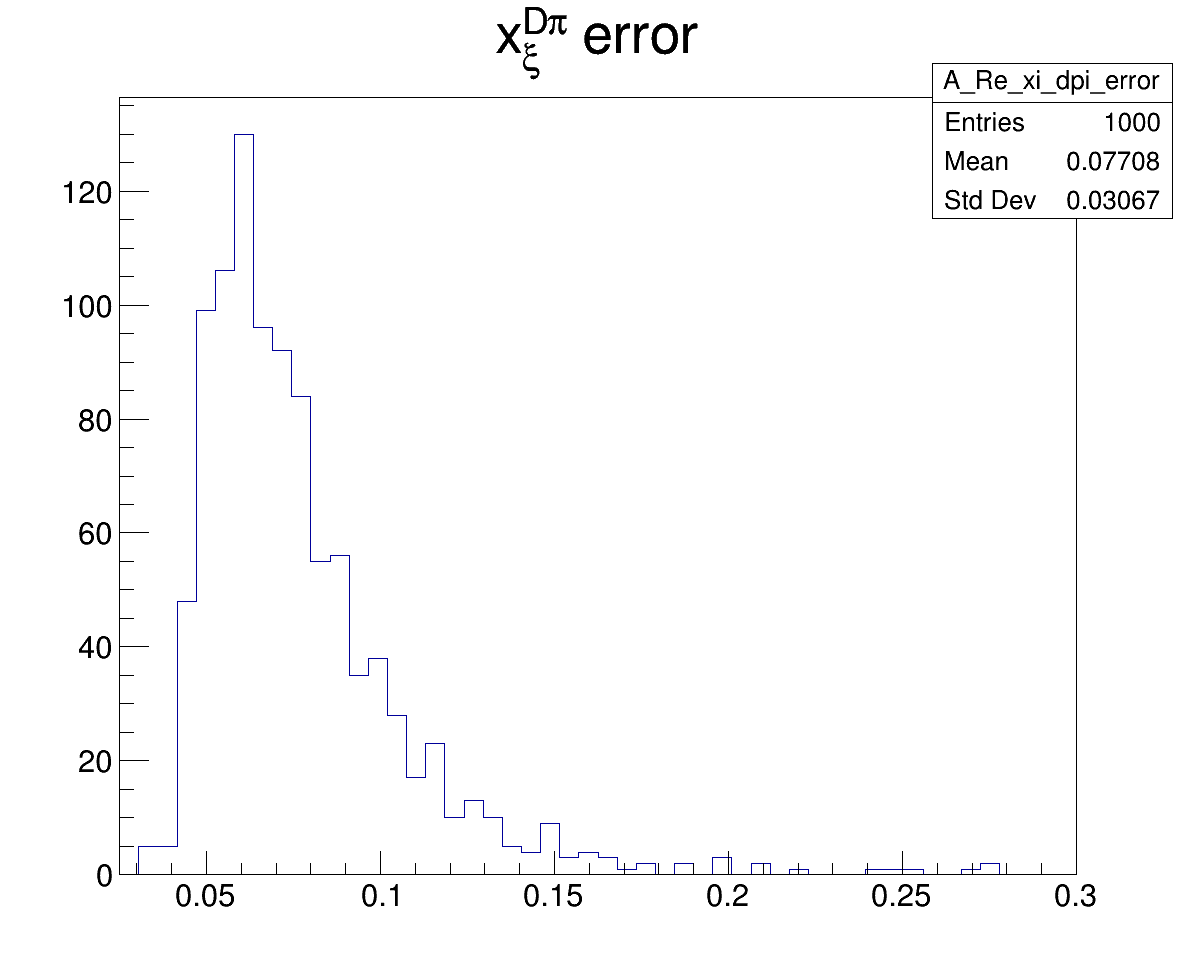
\includegraphics[width = 1.0\textwidth]{Plots/A_Re_xi_dpi_error.png}
      \caption{Error}
    \end{subfigure}%
    \begin{subfigure}{0.25\textwidth}
      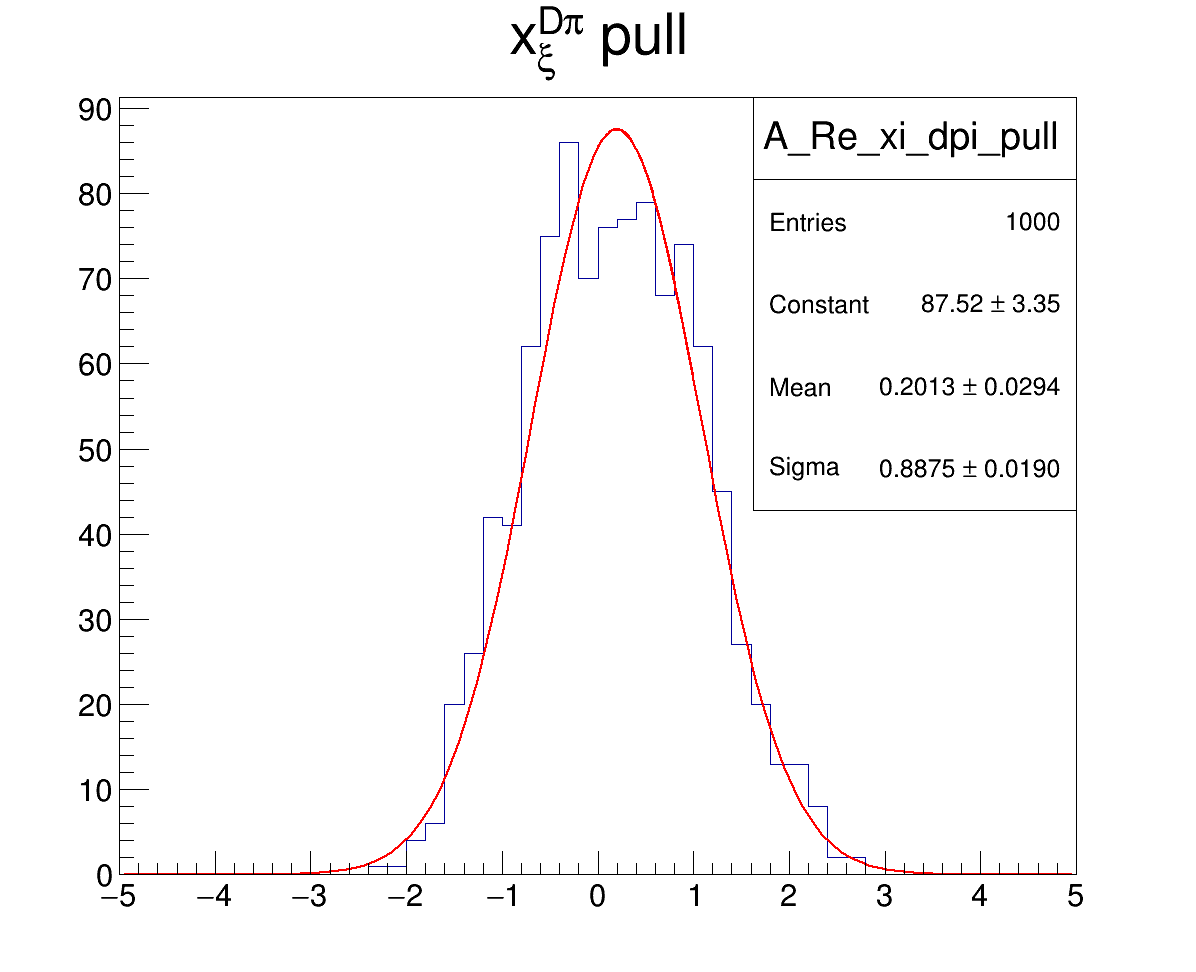
\includegraphics[width = 1.0\textwidth]{Plots/A_Re_xi_dpi_pull.png}
      \caption{Pull}
    \end{subfigure}
    \caption{$x_\xi^{D\pi}$}
  \end{figure}
  \begin{figure}
    \centering
    \vspace{-0.15cm}
    \begin{subfigure}{0.25\textwidth}
      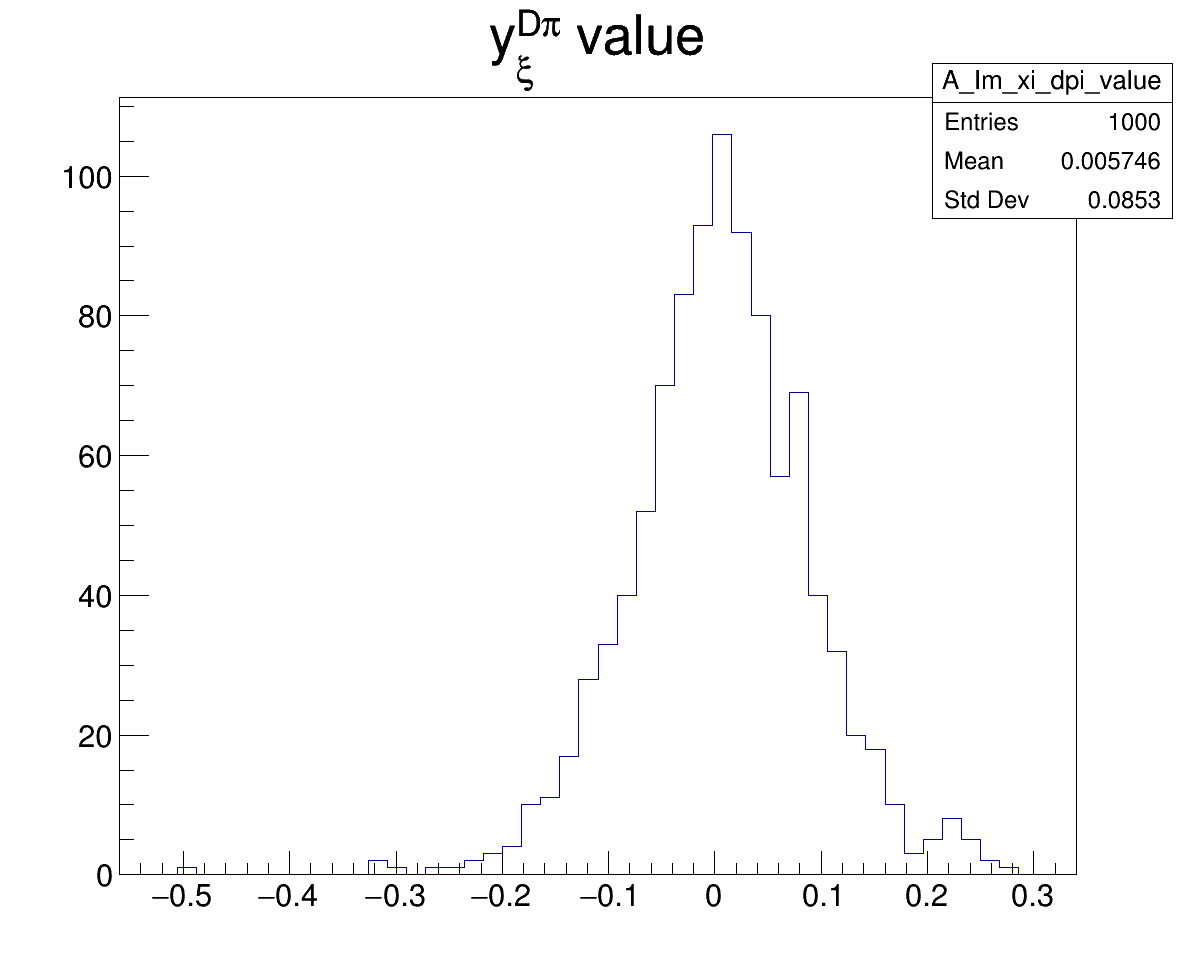
\includegraphics[width = 1.0\textwidth]{Plots/A_Im_xi_dpi_value.png}
      \caption{Value}
    \end{subfigure}%
    \begin{subfigure}{0.25\textwidth}
      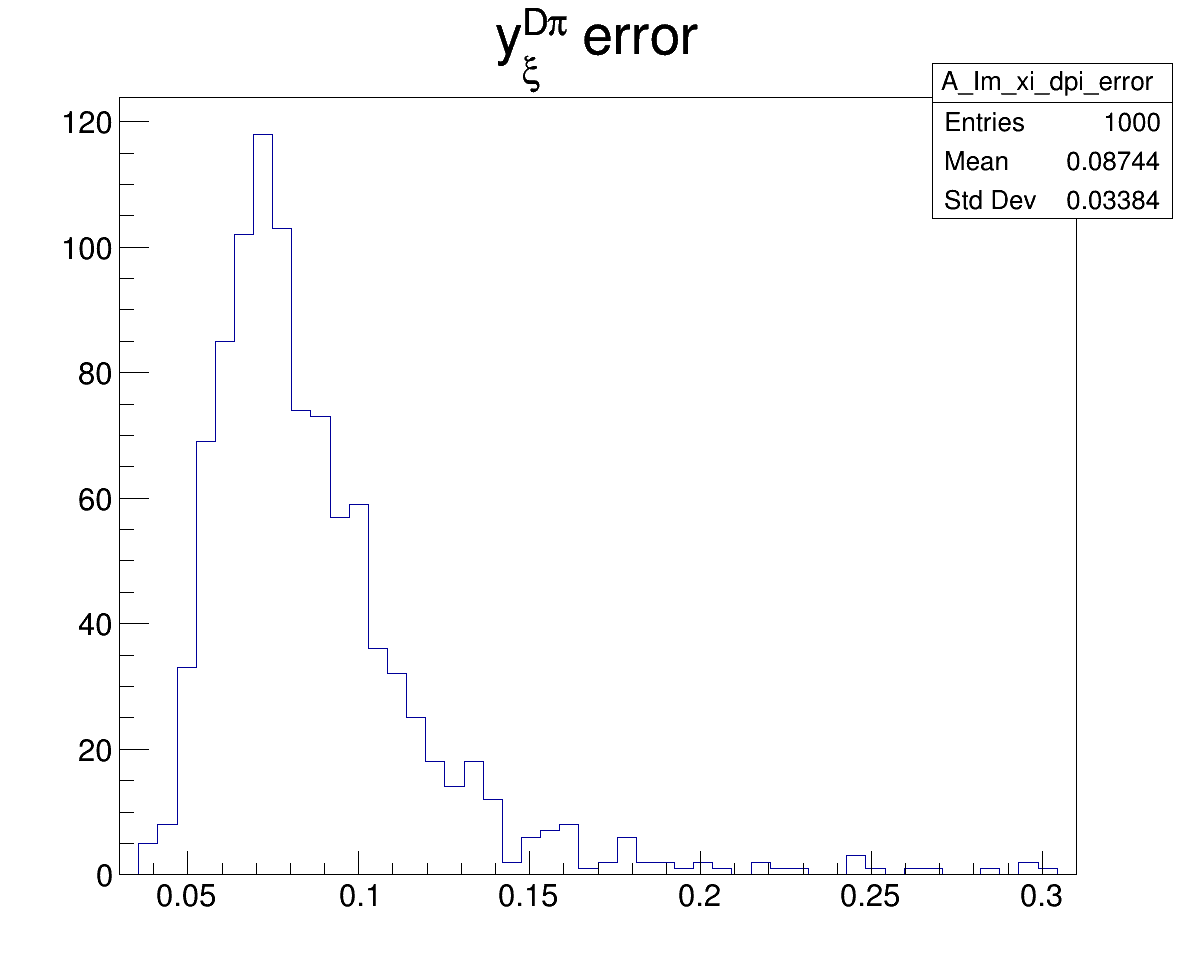
\includegraphics[width = 1.0\textwidth]{Plots/A_Im_xi_dpi_error.png}
      \caption{Error}
    \end{subfigure}%
    \begin{subfigure}{0.25\textwidth}
      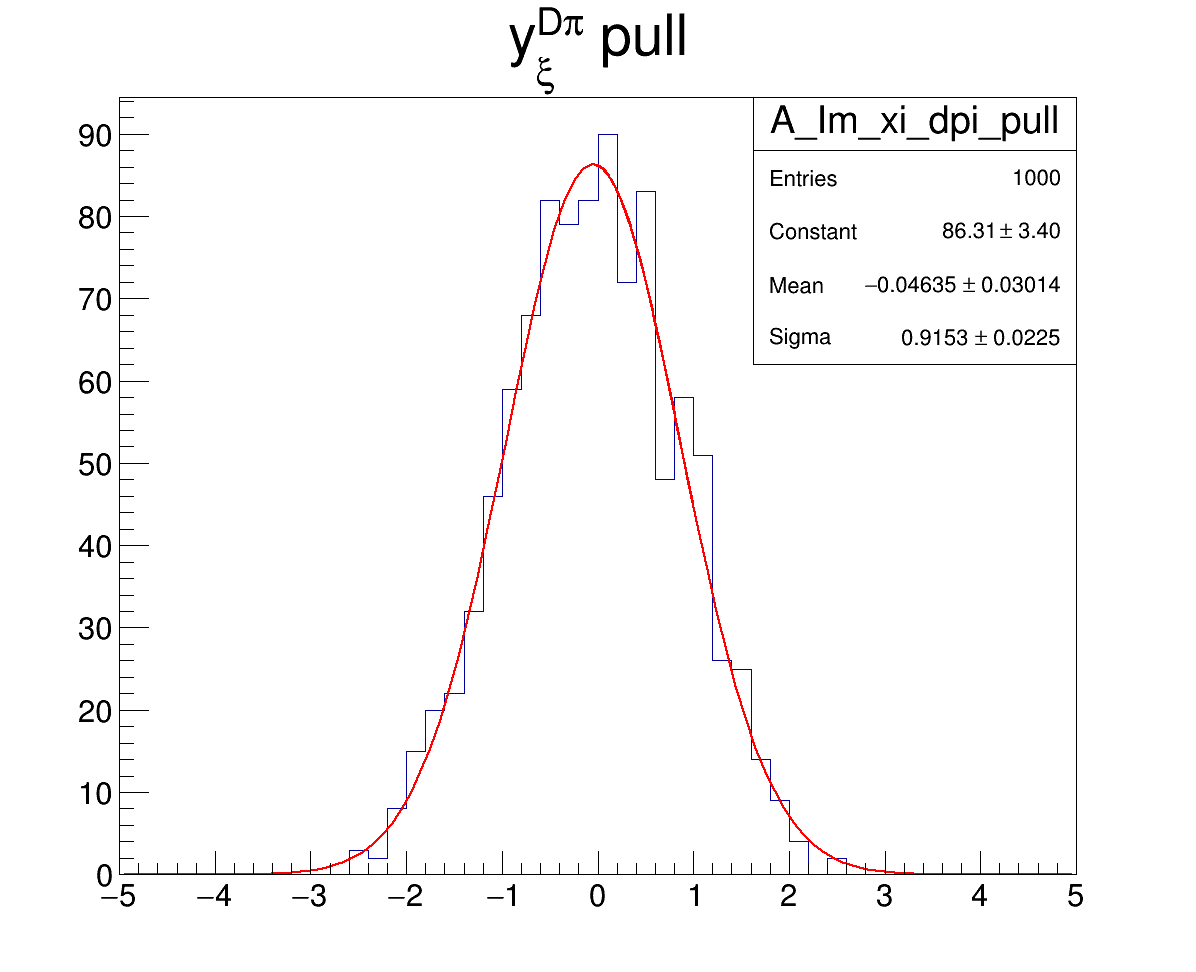
\includegraphics[width = 1.0\textwidth]{Plots/A_Im_xi_dpi_pull.png}
      \caption{Pull}
    \end{subfigure}
    \caption{$y_\xi^{D\pi}$}
  \end{figure}
\end{frame}

\section{GammaCombo}
\begin{frame}{GammaCombo}
  \begin{center}
    {\huge GammaCombo}
  \end{center}
\end{frame}

\begin{frame}{GammaCombo $\delta_B^{DK}$ and $r_B^{DK}$}
  \begin{figure}[H]
    \centering
    \begin{subfigure}{.5\textwidth}
      \centering
      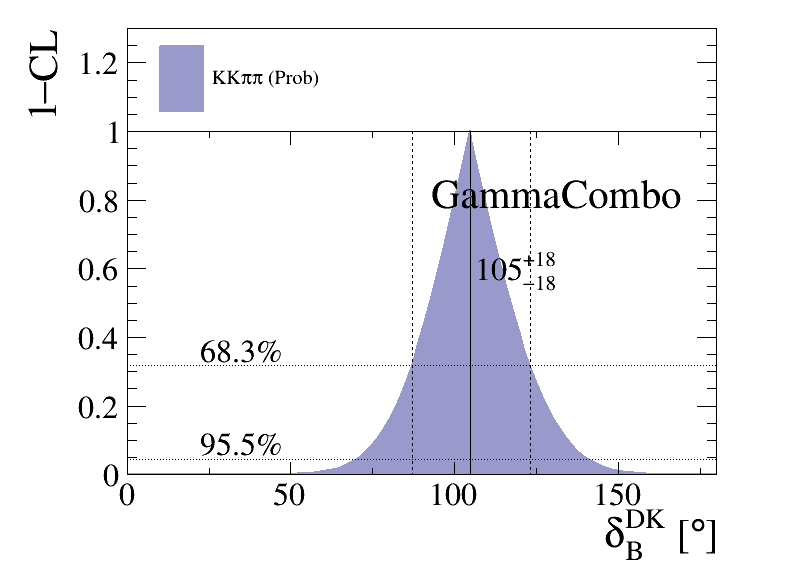
\includegraphics[width=1\linewidth]{Plots/cartesian_cartesian_d_dk.png}
      \caption{$\delta_B^{DK}$}
    \end{subfigure}%
    \begin{subfigure}{.5\textwidth}
      \centering
      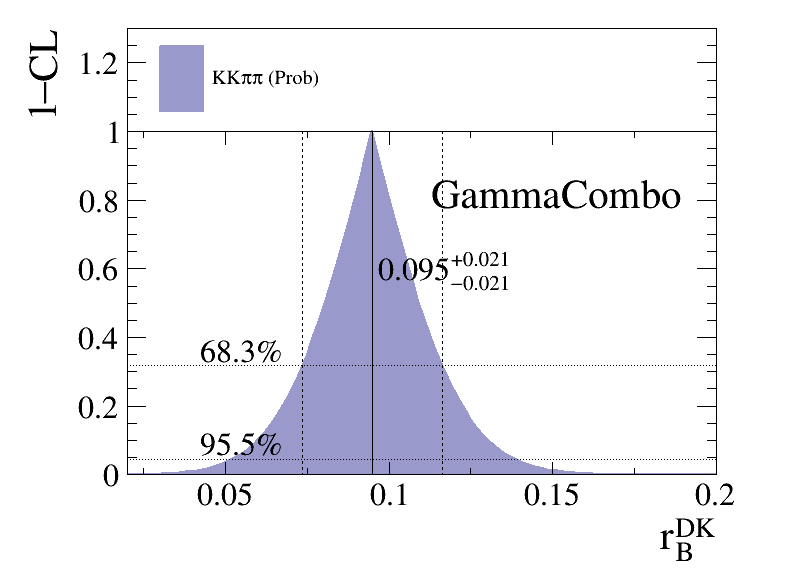
\includegraphics[width=1\linewidth]{Plots/cartesian_cartesian_r_dk.png}
      \caption{$r_B^{DK}$}
    \end{subfigure}
    \caption{}
  \end{figure}
\end{frame}

\begin{frame}{GammaCombo $\delta_B^{D\pi}$ and $r_B^{D\pi}$}
  \begin{figure}[H]
    \centering
    \begin{subfigure}{.5\textwidth}
      \centering
      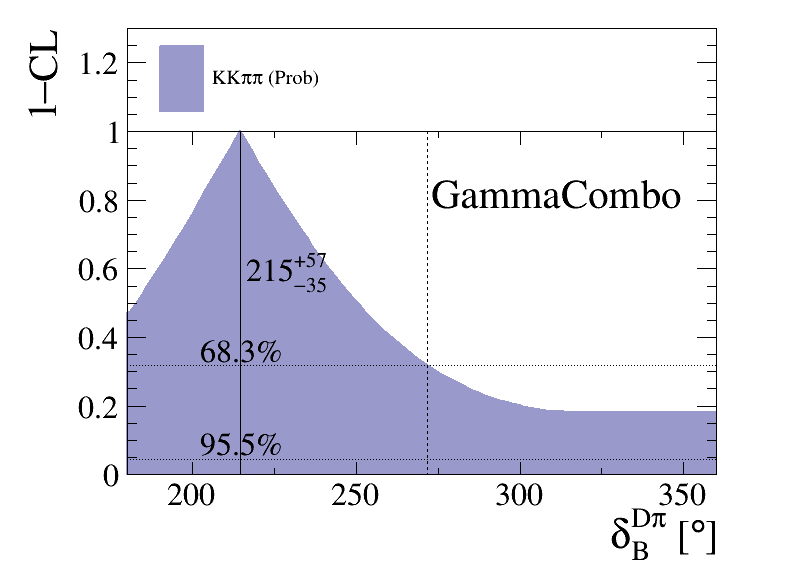
\includegraphics[width=1\linewidth]{Plots/cartesian_cartesian_d_dpi.png}
      \caption{$\delta_B^{D\pi}$}
    \end{subfigure}%
    \begin{subfigure}{.5\textwidth}
      \centering
      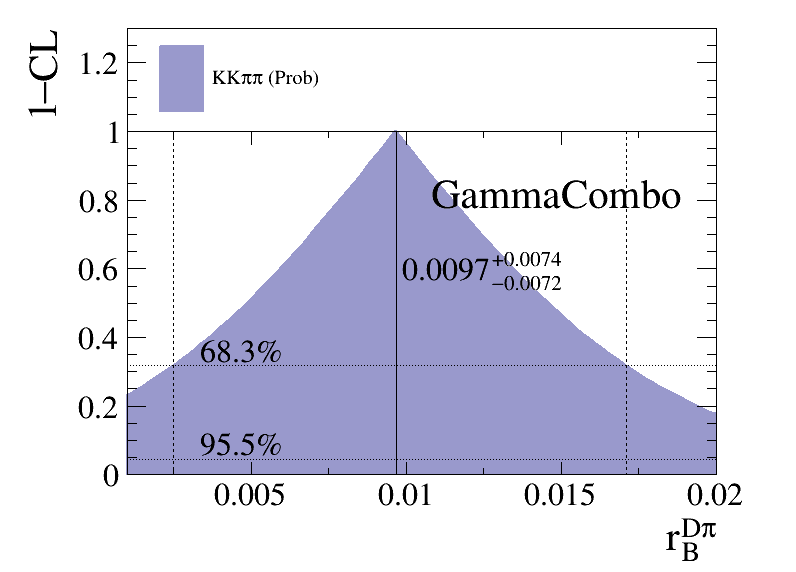
\includegraphics[width=1\linewidth]{Plots/cartesian_cartesian_r_dpi.png}
      \caption{$r_B^{D\pi}$}
    \end{subfigure}
    \caption{}
  \end{figure}
\end{frame}

\begin{frame}{GammaCombo $\gamma$}
  \begin{figure}[H]
    \centering
    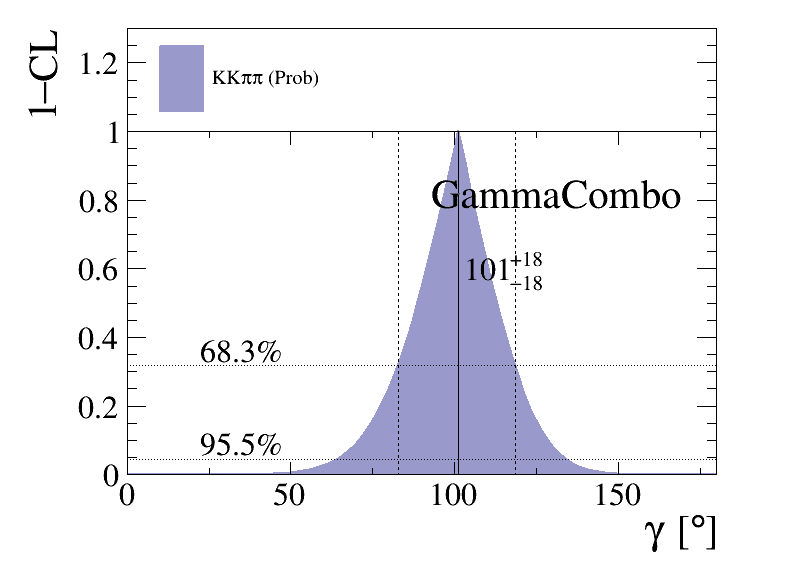
\includegraphics[width=0.8\linewidth]{Plots/cartesian_cartesian_gamma.png}
    \caption{$\gamma$}
  \end{figure}
\end{frame}

\section{Summary}
\begin{frame}{Summary}
  Summary:
  \begin{itemize}
    \item{Global and CP fits are working}
    \item{Toy studies show no suspicious behaviour}
  \end{itemize}
  Next steps:
  \begin{itemize}
    \item{Fine tuning the PDF shape parameters and efficiencies?}
  \end{itemize}
\end{frame}

\begin{frame}{Backup slides: DaVinci error}
  \begin{center}
    DaVinci error message:
  \end{center}
  \begin{figure}
    \includegraphics[width = 1\textwidth]{DaVinciError.png}
  \end{figure}
\end{frame}

\end{document}
